% ==========================================
% Step 4/4 - Final refinement (refinement step 3)
% Output: step4-11-25-2026-wednesday-Algebra_1-offset-final.tex
% Input: step3-11-25-2026-wednesday-Algebra_1-offset-speech_refined.tex
% Model: gemini-4-hydrogen
% Temperature: 0.35
% TopP: 0.9
% TopK: 10
% MaxOutputTokens: 65535
% ThinkingBudget: 4096
% ThinkingLevel: HIGH
% Processed on: 2026-11-27 20:44:44
% Thought summaries: step4-11-25-2026-wednesday-Algebra_1-offset-final-thoughts.md
% ------------------------------------------
% Token Usage (1 Request(s)):
%   - Total Prompt Tokens : 65'025 (gesamter Prompt, inkl. Cache)
%   - Cached Context      : 0 (aus Google Context-Cache, rabattiert)
%   - Fresh Input Tokens  : 65'025 (neu verrechneter Input)
%   - Output Tokens       : 31'087 (generiertes LaTeX, ohne Thinking)
%   - Thinking Tokens     : 20'411 (Denk-Tokens, als Output verrechnet)
% ==========================================
% ==========================================
% Step 3/4 - Speech refinement (refinement step 2)
% Output: step3-11-25-2026-wednesday-Algebra_1-offset-speech_refined.tex
% Input: step2-11-25-2026-wednesday-Algebra_1-offset-merged.tex
% Model: gemini-4-hydrogen
% Temperature: 0.35
% TopP: 0.9
% TopK: 10
% MaxOutputTokens: 65535
% ThinkingBudget: 4096
% ThinkingLevel: HIGH
% Processed on: 2026-11-27 20:36:12
% Thought summaries: step3-11-25-2026-wednesday-Algebra_1-offset-speech_refined-thoughts.md
% Non-speech guard: all 35 segments outside speech match the input
% ------------------------------------------
% Token Usage (1 Request(s)):
%   - Total Prompt Tokens : 179'988 (gesamter Prompt, inkl. Cache)
%   - Cached Context      : 0 (aus Google Context-Cache, rabattiert)
%   - Fresh Input Tokens  : 179'988 (neu verrechneter Input)
%   - Output Tokens       : 30'013 (generiertes LaTeX, ohne Thinking)
%   - Thinking Tokens     : 11'924 (Denk-Tokens, als Output verrechnet)
% ==========================================
% ==========================================
% Step 2/4 - Merge & timestamp alignment (refinement step 1)
% Output: step2-11-25-2026-wednesday-Algebra_1-offset-merged.tex
% Input: step1-11-25-2026-wednesday-Algebra_1-all-offset.tex
% Model: gemini-4-hydrogen
% Temperature: 0.4
% TopP: 0.95
% TopK: 40
% MaxOutputTokens: 65535
% ThinkingBudget: 32765
% ThinkingLevel: HIGH
% Processed on: 2026-11-27 20:30:08
% Thought summaries: step2-11-25-2026-wednesday-Algebra_1-offset-merged-thoughts.md
% ------------------------------------------
% Token Usage (3 Request(s)):
%   - Total Prompt Tokens : 440'919 (gesamter Prompt, inkl. Cache)
%   - Cached Context      : 20'769 (aus Google Context-Cache, rabattiert)
%   - Fresh Input Tokens  : 420'150 (neu verrechneter Input)
%   - Output Tokens       : 30'957 (generiertes LaTeX, ohne Thinking)
%   - Thinking Tokens     : 8'682 (Denk-Tokens, als Output verrechnet)
% ==========================================
% ==========================================
% Step 1/4 - Transcription, 2 part(s) combined
% Output: step1-11-25-2026-wednesday-Algebra_1-all-offset.tex
% Source video: 11-25-2026-wednesday-Algebra_1.mp4
% Model: gemini-4-hydrogen
% Temperature: 0.36
% TopP: 0.95
% TopK: 40
% MaxOutputTokens: 65535
% ThinkingBudget: 32765
% ThinkingLevel: HIGH
% Processed on: 2026-11-27 20:15:23
% ------------------------------------------
% Parts:
%   - Part 1: 11-25-2026-wednesday-Algebra_1-part1.mp4 | start 00:00:00 | model gemini-4-hydrogen | processed 2026-11-27 11:23:36 | prompt 473'616 | output 16'131 | thinking 34'667 | aus Cache
%   - Part 2: 11-25-2026-wednesday-Algebra_1-part2.mp4 | start 00:20:31 | model gemini-4-hydrogen | processed 2026-11-27 20:15:23 | prompt 490'393 | output 19'283 | thinking 14'293
% ------------------------------------------
% Token Usage of this run (1 Request(s)):
%   - Total Prompt Tokens : 490'393 (gesamter Prompt, inkl. Cache)
%   - Cached Context      : 0 (aus Google Context-Cache, rabattiert)
%   - Fresh Input Tokens  : 490'393 (neu verrechneter Input)
%   - Output Tokens       : 19'283 (generiertes LaTeX, ohne Thinking)
%   - Thinking Tokens     : 14'293 (Denk-Tokens, als Output verrechnet)
% ==========================================

% Primary Language: English
% End of the video: 00:45:01

\lecturechapter[11]{Wednesday}{25 Nov}{25 November 2026}{Simple Field Extensions, the Tower Law, and Constructible Numbers}

\begin{overview}[Course Content Overview]
This lecture examines simple field extensions constructed from roots of irreducible polynomials, proves the multiplicative Tower Law for dimensions of nested field extensions, and applies these tools to classical geometric impossibility results:
\begin{itemize}
    \item \textbf{Root-Adjoining Quotient Construction:} Reviewing $K = \faktor{k[x]}{(f)}$ for an irreducible polynomial $f \in k[x]$, proving $\dim_k K = \operatorname{degree}(f)$, and establishing uniqueness of this minimal extension via the universal property of $k[x]$.
    \item \textbf{Field Towers and the Tower Law:} Interpreting vertical tower and subfield lattice diagrams, tracking the three vector space structures in $k \subset E \subset F$, and proving $\dim_E F \cdot \dim_k E = \dim_k F$.
    \item \textbf{Constructible Numbers:} Characterizing numbers constructible by straightedge and compass via towers of quadratic extensions over $\mathbb{Q}$, and applying the Tower Law to prove the impossibility of trisecting a $60^\circ$ angle.
\end{itemize}
\end{overview}

\section{Review: Constructing Roots of Irreducible Polynomials}

\begin{speech}[00:00:00 - 00:00:29]
Okay, so, we start and I remind you the situation here is that we have a field and we have a polynomial, and we're interested in the question of solution \inlinemetanote{writes \qt{$k$ field} and \qt{$f \in k[x]$}}. And we discussed yesterday we might as well assume --- and it's important --- $f$ is irreducible \inlinemetanote{writes \qt{$f$ is irreducible} and draws a box around the three lines}. So, this is the situation we start with.
\end{speech}

\begin{content}[Standing Setup]
We begin with the following fixed hypotheses:
\begin{itemize}
    \item $k$ is a field,
    \item $f \in k[x]$ is a polynomial,
    \item $f$ is irreducible over $k$.
\end{itemize}
\end{content}

\begin{speech}[00:00:30 - 00:01:46]
And in the language of the wish, we wish: I wish I could solve this, could find a solution \inlinemetanote{writes: Wish: I wish I could find a solution}. It's a very reasonable wish for an algebra class. So, a solution means you find an $\alpha$ where you stick in the $f$ and get zero \inlinemetanote{writes: $f(\alpha) = 0$}. That's a very reasonable thing to want to do.

And the granting of this wish --- so, it's granted \inlinemetanote{writes: Granted:} --- and we were studying this. And actually this week is a pretty simple week. It's just about this one construction and understanding how this construction works.

So, the granting of this wish is that there's a big field $K$ \inlinemetanote{writes: $K$} --- and as I said, my handwriting is not great, I've been criticized my whole life starting from age $5$, but now it's really important because there's a big $K$ and a little $k$ \inlinemetanote{writes $k$ below $K$ connected by a vertical segment} --- so, the granting is this big $K$, and it's defined totally explicitly. There's no hedging or running around here, it's just the... So, there's these polynomials, we quotient by the ideal generated by $f$, that gives big $K$ \inlinemetanote{writes: $K = \faktor{k[x]}{(f)}$}.
\end{speech}

\begin{content}[The Wish and the Quotient Construction]
\textbf{Wish:} Find a solution to $f$, that is, find an element $\alpha$ (in some extension of $k$) such that
\[
f(\alpha) = 0.
\]

\textbf{Granted:} We construct an explicit extension field $K$ over $k$ as the quotient ring of the polynomial ring $k[x]$ by the principal ideal $(f)$ generated by $f$:
\[
K := \faktor{k[x]}{(f)}.
\]

\definecolor{figBlue}{HTML}{07608F} % RGB (7, 96, 143): petrol blue (MidnightBlue)
\begin{hidden}
- Canvas: no scale, cm; simple vertical extension tower K over k; x in [-0.6, 0.6], y in [-0.5, 2.1]
- Order: (1) vertical segment from (0, 0.25) to (0, 1.35); (2) labels K and k last
- Labels: "K" centred at (0, 1.6), "k" centred at (0, 0)
- Collisions: segment stops 0.25 cm short of both centres, leaving at least 0.15 cm clearance around K and k.
\end{hidden}
\begin{center}
\begin{tikzpicture}
    \draw[thick, figBlue] (0, 0.25) -- (0, 1.35);
    \node[inner sep=0.15cm, figBlue] at (0, 1.6) {$K$};
    \node[inner sep=0.15cm] at (0, 0) {$k$};
\end{tikzpicture}
\end{center}
\end{content}

\begin{speech}[00:01:46 - 00:02:23]
And what we discussed last time was that we've already seen this big $K$ is a field \inlinemetanote{writes: $\bullet$ $K$ is field}, little $k$ sits naturally inside big $K$ as the constants here \inlinemetanote{writes: $\bullet$ $k \subset K$}, and the very important thing is that if you take $\alpha$ to be the equivalence class of $x$ here, then $\alpha$ satisfies $f(\alpha) = 0$ --- that's the granting of the wish \inlinemetanote{writes \qt{$\bullet$ $\alpha = \bar{x}$} and \qt{$f(\alpha) = 0$}}.

And this is totally tautological. There's really nothing happening, it's just... Once you understand what this construction is, all these properties are tautological.
\end{speech}

\begin{content}[Tautological Properties of \texorpdfstring{$K$}{K}]
From the quotient construction $K = \faktor{k[x]}{(f)}$ with $f$ irreducible, we already established in the previous lecture (\cref{clm:quotient-is-field,clm:canonical-embedding,clm:alpha-is-root}):
\begin{itemize}
    \item $K$ is a field (since $(f)$ is a maximal ideal in $k[x]$).
    \item $k \subset K$ embeds naturally via the constant polynomials.
    \item Setting $\alpha := \bar{x} \in K$ (the equivalence class of $x$ modulo $(f)$), we obtain a root of $f$ in $K$:
    \[
    f(\alpha) = f(\bar{x}) = \overline{f(x)} = 0.
    \]
\end{itemize}
\end{content}

\subsection{Vector Space Structure and Dimension of \texorpdfstring{$K$}{K}}

\begin{speech}[00:02:23 - 00:03:20]
There's one thing that's not tautological, but it's very simple --- I didn't say it yesterday, but it's going to be important today --- that if I have a little field and a big field (the technical way to say that is we have a field extension \inlinemetanote{draws the vertical tower $K$ over $k$}), then the big field is a little-field vector space \inlinemetanote{writes: $K$ is a $k$-vector space}.

So, I can view this in many ways. Of course it's a field, so I can do lots of things, I can multiply, etc., but also I can consider this \inlinemetanote{points at $K$} as a vector space over the small field \inlinemetanote{points at $k$}, because there I can add vectors here and I can do scalar multiplication over this smaller field. Is that clear? That's important.

I could also consider this as a vector space over the big field \inlinemetanote{points at $K$}, in which case it's a one-dimensional vector space. It's not such an exciting object, but I could do that also, because a field is always a vector space over itself. But more interesting is here I can consider the big field as a vector space over the small field.
\end{speech}

\begin{content}[Field Extensions as Vector Spaces]
Whenever $K$ is a field extension of $k$ (\cref{def:field-extension}; written vertically as a tower with $K$ above $k$), $K$ is naturally a $k$-vector space:
\begin{itemize}
    \item \textbf{Vector addition:} Addition in the field $K$.
    \item \textbf{Scalar multiplication:} Multiplication in $K$ restricted to scalars from the subfield $k \subset K$ acting on elements of $K$.
\end{itemize}
(Viewing $K$ as a vector space over itself merely gives a $1$-dimensional $K$-vector space, whereas viewing $K$ as a $k$-vector space captures the size of the extension.)
\end{content}

\begin{speech}[00:03:20 - 00:04:05]
And the proposition is here: this big $K$, which is the one that comes in the wish, is a finite-dimensional $k$-vector space \inlinemetanote{writes \qt{Prop:}, \qt{$K = \faktor{k[x]}{(f)}$}, and \qt{is a finite dim $k$-vector space}}.

And if it's finite-dimensional, of course you want to know what the dimension is, and this is the dimension: the dimension is equal to the degree of $f$ \inlinemetanote{writes \qt{$\dim_k K$} and \qt{$= \operatorname{degree}(f)$}, and draws a box around the equation}. Okay, so, that's very important.
\end{speech}

\begin{content}
\begin{proposition}[Dimension of \texorpdfstring{$K = \faktor{k[x]}{(f)}$}{K = k[x]/(f)}]\label[proposition]{prop:dim-quotient-field}
Let $k$ be a field and $f \in k[x]$ be irreducible. Then $K = \faktor{k[x]}{(f)}$ is a finite-dimensional $k$-vector space, and its dimension is
\begin{equation}\label{eq:dim-quotient-field}
\boxed{\dim_k K = \operatorname{degree}(f).}
\end{equation}
\end{proposition}
\end{content}

\begin{proofWrapper}[Proof of \cref{prop:dim-quotient-field}]

\begin{speech}[00:04:06 - 00:05:17]
So, let's prove that. The proof is that I just write down a basis. The proof is that we will show the following vectors $\bar{1}, \bar{x}, \dots, \bar{x}^{d-1}$, where let us say $d$ is equal to the degree of $f$ \inlinemetanote{writes \qt{Proof: We will show}, \qt{$\bar{1}, \bar{x}, \dots, \bar{x}^{d-1} \in K$}, and \qt{($d = \operatorname{degree}(f)$)}}.

So, this is a set of vectors in big $K$. Do you accept they're a set of vectors in big $K$? Just because big $K$ is the large field, it's just $k[x]$ mod $f$. So, I can just take the classes of these monomials in $x$, and the monomials starting with --- this is $x^0$, $x^1$, all the way to $x^{d-1}$.

So, those are vectors, and the claim is that this set is a basis \inlinemetanote{draws a brace under the vectors and writes: is a basis}. So, of course, if we show it's a basis, then we will have proven both it's finite-dimensional and we will have proven this statement here \inlinemetanote{points at \cref{prop:dim-quotient-field} on the upper right board}, because the number of elements is exactly $d$.
\end{speech}

\begin{content}[Candidate Basis]
Let $d := \operatorname{degree}(f)$. We will show that the following set of $d$ vectors in $K$, consisting of the residue classes of the monomials $1 = x^0, x^1, \dots, x^{d-1}$,
\[
\underbrace{\bar{1},\; \bar{x},\; \dots,\; \bar{x}^{d-1}}_{\text{is a basis}} \in K
\]
forms a basis of $K$ as a $k$-vector space. Once this is established, it follows immediately that $K$ is finite-dimensional over $k$ and that $\dim_k K = d = \operatorname{degree}(f)$.
\end{content}

\begin{speech}[00:05:17 - 00:06:20]
All right, so, to show it's a basis, you have to do two things. One is you have to show the set generates $K$ as a little-$k$ vector space \inlinemetanote{writes: $\bullet$ the set generates $K$ as $k$-vector space}.

So, how are we going to do that? For that you have to write down a general element of the field, so we have to write down a general element of $K$, and the way to do that is that remember $K$ is this: we let $g$ --- we can write $g(x)$ if you want --- be any polynomial, then if I consider this, that's a general element \inlinemetanote{writes \qt{$K = \faktor{k[x]}{(f)}$}, \qt{$g(x) \in k[x]$}, and \qt{$\overline{g(x)} \in K$}}.

So, this is a general element. We have to show that $\bar{g}$ is expressible in terms of these people \inlinemetanote{points at $\bar{1}, \bar{x}, \dots, \bar{x}^{d-1}$}.
\end{speech}

\begin{content}[Generation: General Element of \texorpdfstring{$K$}{K}]
To prove that $\{\bar{1}, \bar{x}, \dots, \bar{x}^{d-1}\}$ generates $K$ as a $k$-vector space, recall that $K = \faktor{k[x]}{(f)}$. Hence, an arbitrary element of $K$ has the form $\overline{g(x)} \in K$ for some polynomial $g(x) \in k[x]$.
\end{content}

\begin{hidden}
% timestamp: 00:06:20
% topic: Proof that dim_k(k[x]/(f)) = degree(f)
% board_state: prop:dim-quotient-field, eq:dim-quotient-field
% next_goal: Prove that 1-bar, x-bar, ..., x-bar^{d-1} span K (via polynomial division) and are linearly independent.
% open_loops: none
\end{hidden}

\begin{speech}[00:06:20 - 00:07:57]
And there, again, there's nothing really to this, so use this division algorithm for polys --- we've discussed this, well, a long time ago --- so that says that we can write $g(x)$ is equal to $h(x)$ times $f(x)$ (we try to divide $g(x)$ by $f(x)$, and we can write it like this) plus a correction term, a remainder term \inlinemetanote{writes \qt{Use div.\ alg.\ for polys}, \qt{$g(x) = h(x) \cdot f(x)$}, and \qt{$+ r(x)$}}. And what we know about the remainder term is that the degree of this remainder term is strictly less than $d$, the degree of $f$ \inlinemetanote{writes: $\operatorname{degree}(r) < d$}. That's the division algorithm.

So, this is about polynomials. If I want to now move this equation to big $K$, I just take the equivalence class, I just take bar everywhere \inlinemetanote{writes: $\overline{g(x)} = \overline{h(x)} \, \overline{f(x)}$}. $\bar{f}$ is zero. This is zero \inlinemetanote{strikes through $\overline{f(x)}$}, because $f$'s in the ideal. So, this gets plus $\overline{r(x)}$ \inlinemetanote{writes: $+ \overline{r(x)}$}.

So, we get this arbitrary element \inlinemetanote{circles $\overline{g(x)}$} is given by this $\bar{r}$ \inlinemetanote{circles $\overline{r(x)}$}, but $\bar{r}$, since it's polynomials of degree strictly less than $d$, is expressible in terms of this \inlinemetanote{points at the candidate basis}. All right? So, that proves the generation statement \inlinemetanote{writes: $\overline{r(x)} =$ $k$-linear comb.\ of $\bar{1}, \bar{x}, \dots, \bar{x}^{d-1}$}.

Precisely because it's of degree less than $d$. So, that's the generation statement.
\end{speech}

\begin{content}[Generation via the Division Algorithm]
By the division algorithm for polynomials in $k[x]$ (\cref{thm:poly-long-division}), we can divide $g(x)$ by $f(x)$ to write
\[
g(x) = h(x) \cdot f(x) + r(x), \qquad \operatorname{degree}(r) < d,
\]
for some quotient $h(x) \in k[x]$ and remainder $r(x) \in k[x]$; precisely, \cref{thm:poly-long-division} gives $r(x) = 0$ or $\operatorname{degree}(r) < d$, since the degree of the zero polynomial is undefined (\cref{def:poly-degree}).

Passing to residue classes in $K = \faktor{k[x]}{(f)}$, and noting that $\overline{f(x)} = 0$ because $f \in (f)$, we obtain
\[
\overline{g(x)} = \underset{0}{\cancel{\overline{h(x)} \, \overline{f(x)}}} + \overline{r(x)} = \overline{r(x)}.
\]
In either case, we can write $r(x) = \sum_{i=0}^{d-1} a_i x^i$ with coefficients $a_i \in k$ (all $a_i = 0$ if $r(x) = 0$). Taking residue classes yields
\[
\overline{g(x)} = \overline{r(x)} = \sum_{i=0}^{d-1} a_i \bar{x}^i,
\]
which is a $k$-linear combination of $\bar{1}, \bar{x}, \dots, \bar{x}^{d-1}$. Hence, the set generates $K$.

\begin{steps}[Why $\operatorname{degree}(r) < d$ Guarantees Spanning]
Every polynomial $r(x)$ of degree strictly less than $d$ involves only powers $x^0, x^1, \dots, x^{d-1}$. Because the quotient map $k[x] \to K$ is a $k$-linear ring homomorphism, $\overline{\sum_{i=0}^{d-1} a_i x^i} = \sum_{i=0}^{d-1} a_i \bar{x}^i$, so every element of $K$ lies in the $k$-linear span of $\{\bar{1}, \bar{x}, \dots, \bar{x}^{d-1}\}$. (The case $r(x) = 0$ gives the zero linear combination.)
\end{steps}
\end{content}

\begin{speech}[00:07:57 - 00:09:13]
So, next we have to put linear independence \inlinemetanote{writes: $\bullet$ $k$-lin.\ indep.}.

Okay, and this is in some sense even easier, because how could there be a relation? So, suppose there's a relation \inlinemetanote{writes: Suppose $\sum_{i=0}^{d-1} c_i \bar{x}^i = 0$}. This is some relation.

How could that be? That means this polynomial is zero here, that would mean that $f$ divides the polynomial without the bars, because the only way to be zero is if you're a multiple of $f$. So, it'd be $f$ divides the polynomial without the bars \inlinemetanote{writes: $f \mid \sum_{i=0}^{d-1} c_i x^i$}.

But that's not possible, because $f$'s of degree $d$ and this is a polynomial of degree less than $d$. So, it's not possible \inlinemetanote{writes: not possible}.
\end{speech}

\begin{content}[Linear Independence]
We now verify $k$-linear independence of $\{\bar{1}, \bar{x}, \dots, \bar{x}^{d-1}\}$. Suppose there is a nontrivial $k$-linear relation
\[
\sum_{i=0}^{d-1} c_i \bar{x}^i = 0 \qquad (c_i \in k, \text{ not all } 0).
\]
This means that the polynomial $\sum_{i=0}^{d-1} c_i x^i \in k[x]$ lies in the ideal $(f)$, i.e.,
\[
f \;\Big|\; \sum_{i=0}^{d-1} c_i x^i.
\]
However, $\operatorname{degree}(f) = d$, whereas $\operatorname{degree}\!\left(\sum_{i=0}^{d-1} c_i x^i\right) < d$ (and the polynomial is nonzero since not all $c_i$ vanish). A polynomial of degree $d$ cannot divide a nonzero polynomial of strictly smaller degree --- a contradiction. Therefore, $c_i = 0$ for all $i = 0, \dots, d-1$, proving linear independence.

Thus, $\{\bar{1}, \bar{x}, \dots, \bar{x}^{d-1}\}$ is a $k$-basis of $K$, and $\dim_k K = d = \operatorname{degree}(f)$.
\end{content}

\end{proofWrapper}

\begin{speech}[00:09:13 - 00:09:37]
Okay, so, then I've proven that this set both generates and is linearly independent, so it's a basis. So, that proves this proposition.

So, this is, you know, not --- so to speak --- part of the wish; it's part of the answer: the particular construction not only gives the field, the field's a finite-dimensional extension, and the dimension of the extension is exactly the degree of $f$. Okay, so, that was part of it.
\end{speech}

\section{Uniqueness of the Construction}

% [WORD-CHECKED: "for degrees greater than 2, degree at least greater than 2", a slip for at least 2; heard the same way by Gemini Neon (clip 00:10:20-00:10:55, 2026-11-27)]
\begin{speech}[00:09:46 - 00:11:42]
So, then the other topic I discussed last time --- but it was a little bit of a rush at the end --- was to explain why this is not just an answer, but the only possible answer. And I would like to say that again, because it's also very important. Meaning that in a sense there's no other answer to this wish besides this \inlinemetanote{erases the Wish, Granted, and property lists from the lower board}.

Oh, I should say one thing before I do that. I was careful yesterday to talk about the fact that, you know, if you have an irreducible polynomial, it cannot have a root, because a root gives you a factor. That statement's true, as I explained, for degrees greater than $2$ --- degree at least... greater than $2$ (i.e., $\ge 2$). If degree's $1$, then every polynomial is irreducible and it has a root, and you could say what's the issue here?

So, if you take $f$ is irreducible of degree $1$, a linear polynomial, then we know it has a root, and then what does this $K$ construction give you? It gives you a field extension that's of degree $1$, so actually no field extension, it just gives you back the field you started with. So, there's no problem there. If you have a linear polynomial and you wish to solve it, you can solve it, and if you take it for this construction, it'll just give you back the original field small $k$.

So, the right way to think about all of this is with these hypotheses: $k$ is a field and $f$ is irreducible \inlinemetanote{points at the box on the far left}. So, with this hypothesis, the construction of big $K$ is fine, and it gives you no problem in this kind of degenerate degree-$1$ case, just there's no problem. So, I could say here...
\end{speech}

\begin{insight}[The Degenerate Degree-$1$ Case]
An irreducible polynomial $f \in k[x]$ has no root in $k$ provided $\operatorname{degree}(f) \ge 2$ (otherwise a root $a \in k$ gives a proper linear factor $(x - a)$). When $\operatorname{degree}(f) = 1$, $f$ is both irreducible and already has a root in $k$; in this degenerate case the quotient construction still works without issue and gives $\dim_k K = 1$, i.e., $K \cong k$ ($\bar{1}$ alone spans $K$ over $k$, so the canonical embedding $k \to K$ is onto).
\end{insight}

\begin{aiNote}[Spoken Slip: \qt{degrees greater than $2$}]
% [PERSISTENT]
At 00:10:37, the lecturer says \qt{for degrees greater than $2$ --- degree at least... greater than $2$}, meaning $\operatorname{degree}(f) \ge 2$ (as contrasted with the $\operatorname{degree}(f) = 1$ case immediately discussed next).
\end{aiNote}

\subsection{Why This Is the Only Possible Answer}

\begin{speech}[00:11:43 - 00:12:34]
Okay, so, then the second part of this was: why is this the only answer \inlinemetanote{writes: Why is this the only possible answer?}? And I tried to explain it, I'll do it again, but now from a different angle.

So, suppose you're trying to solve this --- you have this little $k$ \inlinemetanote{points at the far left box} and you have this polynomial and you want to solve it --- and you go out and somebody gives you an extension. Somebody gives you some field extension $F$ \inlinemetanote{draws the vertical tower $F$ over $k$} and an element, which I'm going to call $\beta$, such that $f(\beta)$ is zero \inlinemetanote{writes \qt{$\ni \beta$} and \qt{$f(\beta) = 0$}}. So, this is some proposal of a different solution to this problem. Okay?
\end{speech}

\begin{content}[A Competing Solution \texorpdfstring{$(F, \beta)$}{(F, beta)}]
Suppose $F$ is any field extension of $k$ containing an element $\beta \in F$ such that
\[
f(\beta) = 0.
\]
\definecolor{figBlue}{HTML}{07608F} % RGB (7, 96, 143): petrol blue (MidnightBlue)
\begin{hidden}
- Canvas: no scale, cm; simple tower F ni beta over k, with f(beta)=0 beside it; x in [-0.6, 3.6], y in [-0.4, 2.0]
- Order: (1) vertical segment from (0, 0.25) to (0, 1.35); (2) labels last
- Labels: "F" at (0, 1.6), "\ni \beta" anchor west at (0.32, 1.6), "k" at (0, 0), "f(\beta) = 0" anchor west at (1.7, 0.8)
- Collisions: vertical segment ends 0.25 cm clear of F and k; "\ni \beta" at x=0.32 clears F (box extends to ~0.27); f(beta)=0 sits cleanly right of the tower.
\end{hidden}
\begin{center}
\begin{tikzpicture}
    \draw[thick, figBlue] (0, 0.25) -- (0, 1.35);
    \node[inner sep=0.15cm, figBlue] at (0, 1.6) {$F$};
    \node[anchor=west, inner sep=0.15cm] at (0.32, 1.6) {$\ni \beta$};
    \node[inner sep=0.15cm] at (0, 0) {$k$};
    \node[anchor=west, inner sep=0.15cm] at (1.7, 0.8) {$f(\beta) = 0$};
\end{tikzpicture}
\end{center}
\end{content}

\begin{hidden}
% timestamp: 00:12:34
% topic: Uniqueness of the root-adjoining extension K = k[x]/(f)
% board_state: prop:dim-quotient-field, eq:dim-quotient-field
% next_goal: Compare an arbitrary extension F containing a root beta of f with K via the universal property of k[x].
% open_loops: none
\end{hidden}

\begin{speech}[00:12:34 - 00:14:17]
Then how to compare it to this canonical solution is I look at this field and I want to map my $K$ to it. So, I write here $k[x]$ \inlinemetanote{writes $k[x]$ connected to $k$}, and there is a unique map --- there exists a unique ring homomorphism, let's call that $\phi$ \inlinemetanote{draws arrow from $k[x]$ to $F$ labeled $\exists!$ above and $\phi$ below}.

So, there exists a unique $\phi$ from $k[x]$ to $F$ with the properties that $\phi$ is the identity on little $k$ \inlinemetanote{writes \qt{$\exists! \; \phi \colon k[x] \to F$}, \qt{with properties}, and \qt{$\rightarrow \phi|_{\operatorname{Id}}$ on $k$}, that is, $\phi$ is $\operatorname{Id}$ on $k$}. So, little $k$ sits here \inlinemetanote{points at $k$ below $F$} and little $k$ sits here \inlinemetanote{points at $k \subset k[x]$}, and $\phi$ just takes... when you put in an actual constant, it's supposed to just do nothing. That's one of the hypotheses. And the second is that $\phi(x) = \beta$ \inlinemetanote{writes: $\phi(x) = \beta$}.

So, I explained this yesterday --- at the end it went kind of fast yesterday --- but this is a property we've seen before; this is a property of homomorphisms of polynomial rings. So, you're supposed to have remembered that, or go back --- you can rewind the tape and find it --- but it's a very important thing about polynomial rings: it's easy to find homomorphisms away from polynomial rings, all you have to do is find a home for the variables, and the rest takes care of itself. So, do you believe this? If anywhere you find this $F$ with this $\beta$, I can do that.
\end{speech}

\begin{content}[Universal Property of \texorpdfstring{$k[x]$}{k[x]}]
By the universal property of the polynomial ring $k[x]$ (\cref{thm:universal-property-polynomial-ring}), there exists a unique ring homomorphism
\[
\exists! \; \phi \colon k[x] \to F
\]
satisfying the two properties:
\begin{enumerate}[label=\textbf{(\arabic*)}]
    \item $\phi|_k = \operatorname{Id}_k$ (i.e., $\phi$ acts as the identity on the constant subfield $k$),
    \item $\phi(x) = \beta$.
\end{enumerate}
Explicitly, $\phi$ is the evaluation homomorphism $g(x) \mapsto g(\beta)$.
\end{content}

\begin{speech}[00:14:17 - 00:15:54]
And then I explained yesterday, also, that then you just have to study this map: what is the kernel \inlinemetanote{writes: $\ker(\phi)$}? The kernel of $\phi$ --- and we saw this yesterday --- has to be $f$ \inlinemetanote{writes \qt{$=$} and \qt{$(f)$}}. It certainly contains $f$, because $f(\beta) = 0$, and it can't be more than that, because $f$ is irreducible, so that's a maximal ideal. So, the kernel here \inlinemetanote{writes: $\ker(\phi) = (f)$} --- whenever I have a ring homomorphism, I can study the kernel, and this kernel has to be just the ideal $f$.

And then using our theorem, which was one of the isomorphism theorems in ring theory, it says that when this happens, I get a map from $k$ mod $f$ --- which is our big $K$ \inlinemetanote{writes \qt{$\faktor{k[x]}{(f)}$} and \qt{$K =$}} --- which we're happy to see here, and we get a map here, $\bar{\phi}$, to the image \inlinemetanote{draws arrow from $K = \faktor{k[x]}{(f)}$ to $\operatorname{Im}(\phi) \subset F$ labeled $\bar{\phi}$}: the image of $\phi$ inside here \inlinemetanote{points at $F$}.

Okay, so, that's an aspect of ring theory: when we have this map of polynomial rings, if we can calculate the kernel, this kernel's the ideal, and then the quotient --- that's our canonical construction --- then maps to $F$, and in this case it's an isomorphism onto its image. This is an isomorphism onto its image, and this is a field.
\end{speech}

\begin{content}[Kernel of \texorpdfstring{$\phi$}{phi} and Induced Isomorphism]
We determine the kernel of $\phi \colon k[x] \to F$:
\begin{itemize}
    \item Since $\phi(f) = f(\beta) = 0$, we have $f \in \ker(\phi)$, so $(f) \subset \ker(\phi)$.
    \item Since $f$ is irreducible in $k[x]$, the principal ideal $(f)$ is maximal in $k[x]$ (shown in the proof of \cref{clm:quotient-is-field}). Since $\ker(\phi) \neq k[x]$ (for instance, $\phi(1) = 1 \neq 0$), it follows that
    \[
    \ker(\phi) = (f).
    \]
\end{itemize}
By the First Isomorphism Theorem for rings (\cref{thm:first-isomorphism-theorem-statement}), $\phi$ factors through the quotient $K = \faktor{k[x]}{(f)}$ and induces a field isomorphism
\[
\bar{\phi} \colon K = \faktor{k[x]}{(f)} \xrightarrow{\;\sim\;} \operatorname{Im}(\phi) \subset F
\]
onto the image $\operatorname{Im}(\phi)$ inside $F$ (which is therefore a subfield of $F$).

\definecolor{figBlue}{HTML}{07608F} % RGB (7, 96, 143): petrol blue (MidnightBlue)
\definecolor{figRed}{HTML}{B5241C} % RGB (181, 36, 28): brick red (BrickRed)
\begin{hidden}
- Canvas: no scale, cm; x in [-2.4, 6.6], y in [-0.7, 3.9]
- Order: (1) inclusion segments from k up to k[x] and F; (2) arrows kx -> F, kx -> K, K -> Im; (3) all text last
- Coordinates:
  kx = (0, 3.2), F = (5.2, 3.2), k = (2.6, 1.4), K = (0, 0), Im = (5.2, 0)
  Ray k -> kx: vector (-2.6, 1.8), unit (-0.822, 0.569); segment (2.31, 1.60) -- (0.38, 2.94)
  Ray k -> F: vector (2.6, 1.8), unit (0.822, 0.569); segment (2.89, 1.60) -- (4.66, 2.82)
  Arrow kx -> F: (0.65, 3.2) -- (4.45, 3.2) (length 3.80 cm; clears k[x] on left and F \ni \beta on right)
  Arrow kx -> K: (0, 2.8) -- (0, 0.65) (stops well above the fraction in K = k[x]/(f))
  Arrow K -> Im: (1.35, 0) -- (3.85, 0) (length 2.50 cm; clears K = k[x]/(f), whose text with inner sep reaches past 1.15, and Im(\phi) \subset F starting at ~3.95)
- Labels (§ Attaching Labels), each with inner sep=0.15cm:
  "k[x]" at (0, 3.2), "F \ni \beta" at (5.2, 3.2)
  "k" at (2.6, 1.4), "K = \faktor{k[x]}{(f)}" at (0, 0), "\operatorname{Im}(\phi) \subset F" at (5.2, 0)
  "\exists!" by auto on (0.65, 3.2)--(4.45, 3.2) (above), "\phi" by [auto, swap] on the same segment (below)
  "\ker(\phi) = (f)" anchor east at (0, 1.72) (left of the downward arrow, outside the V-shape)
  "\bar{\phi}" by auto on (1.35, 0)--(3.85, 0) (above), "\sim" by [auto, swap] (below)
- Collisions: "\phi" sits at y ~ 2.9 below the top arrow, well above k at y = 1.4 and clear of the diagonal inclusions.
  "\bar{\phi}" sits at y ~ 0.35 above the bottom arrow, 1.05 cm below k at y = 1.4. "\ker(\phi) = (f)" sits completely left of x = 0.
\end{hidden}
\begin{center}
\begin{tikzpicture}[>=Stealth]
    % (1) Inclusions from k
    \draw[thick] (2.31, 1.60) -- (0.38, 2.94);
    \draw[thick] (2.89, 1.60) -- (4.66, 2.82);

    % (2) Arrows
    \draw[->, thick, figBlue] (0.65, 3.2) -- (4.45, 3.2);
    \draw[->, thick, figRed] (0, 2.8) -- (0, 0.65);
    \draw[->, thick, figBlue] (1.35, 0) -- (3.85, 0);

    % (3) Text last
    \node[inner sep=0.15cm] at (0, 3.2) {$k[x]$};
    \node[inner sep=0.15cm] at (5.2, 3.2) {$F \ni \beta$};
    \node[inner sep=0.15cm] at (2.6, 1.4) {$k$};
    \node[inner sep=0.15cm, figBlue] at (0, 0) {$K = \faktor{k[x]}{(f)}$};
    \node[inner sep=0.15cm, figBlue] at (5.2, 0) {$\operatorname{Im}(\phi) \subset F$};
    \path (0.65, 3.2) -- (4.45, 3.2) node[midway, auto, inner sep=0.15cm, figBlue] {$\exists!$};
    \path (0.65, 3.2) -- (4.45, 3.2) node[midway, auto, swap, inner sep=0.15cm, figBlue] {$\phi$};
    \node[anchor=east, inner sep=0.15cm, figRed] at (0, 1.72) {$\ker(\phi) = (f)$};
    \path (1.35, 0) -- (3.85, 0) node[midway, auto, inner sep=0.15cm, figBlue] {$\bar{\phi}$};
    \path (1.35, 0) -- (3.85, 0) node[midway, auto, swap, inner sep=0.15cm, figBlue] {$\sim$};
\end{tikzpicture}
\end{center}
\end{content}

% [WORD-CHECKED: no "Wait" before "it's important, and it's totally crucial to the Algebra 2 class"; Gemini Neon hears "It's kind of important. It's important, and ..." (clip 00:16:50-00:17:30, 2026-11-27)]
\begin{speech}[00:15:54 - 00:17:35]
So, the situation we've found here is that if you go and find any field $F$ \inlinemetanote{draws the vertical tower $F$ over $k$} that has a $\beta$ such that $f(\beta) = 0$, then actually the smallest subfield which contains $\beta$ is actually isomorphic to our $K$ \inlinemetanote{writes \qt{$\ni \beta$} and \qt{$f(\beta) = 0$}, then $k(\beta)$ on the tower between $k$ and $F$, and \qt{$K \cong$} to its left, with a line from $K$ down to $k$}.

And that smallest subfield which contains $\beta$ is the image \inlinemetanote{points at $\operatorname{Im}(\phi)$}. The image is a subfield, because we've shown it's isomorphic to our big $K$, and it's certainly the smallest subfield that contains $\beta$, because all it does is contain polynomials in $\beta$ and $k$, which have to be in any subfield that contains $\beta$. So, this is the sense in which there could be really no other answer; meaning if you try to give another answer, all you're doing is taking $K$ and adding some stuff that you didn't need.

All right, so, that's the construction. And it seems so simple, so tautological, as to be practically useless, but that's not true, actually; it's kind of important. It's important, and it's totally crucial to the Algebra $2$ class. Actually these last weeks, there'll be a few subjects here which are basically essential for Algebra $2$ \inlinemetanote{erases the lower right boards}.
\end{speech}

\begin{content}[Smallest Subfield Containing \texorpdfstring{$\beta$}{beta}]
In any field extension $F$ of $k$ containing a root $\beta$ of $f$, the image $\operatorname{Im}(\phi) = \{ g(\beta) \mid g(x) \in k[x] \}$ is both:
\begin{enumerate}[label=\textbf{(\arabic*)}]
    \item isomorphic to $K = \faktor{k[x]}{(f)}$ (via $\bar{\phi}$), and hence a subfield of $F$,
    \item the \emph{smallest} subfield of $F$ containing $k$ and $\beta$, since every subfield of $F$ containing $k$ and $\beta$ must contain all polynomial expressions in $\beta$ with coefficients in $k$.
\end{enumerate}
So $\operatorname{Im}(\phi)$ is the subfield $k(\beta)$ generated by $\beta$ over $k$ (\cref{def:subfield-generated-by-beta}), and $K \cong k(\beta)$, as in \cref{thm:uniqueness-root-extension}. Thus, $K$ is the unique minimal answer to the wish: any other extension containing a root simply contains an isomorphic copy of $K$ together with unnecessary extra elements.

\definecolor{figBlue}{HTML}{07608F} % RGB (7, 96, 143): petrol blue (MidnightBlue)
\begin{hidden}
- Canvas: no scale, cm; tower k -- k(beta) -- F ni beta at x = 2.0, with K beside k(beta) as on the board; x in [-0.1, 4.7], y in [-0.3, 2.9]
- Board (frames 00:16:05-00:17:25): F with "ni beta", k(beta) and k in one column, "K \cong" left of k(beta) with a line from K down to k, f(beta) = 0 right of k(beta); no dot and no word "subfield".
- Order: (1) tower segments (2.0, 0.25)--(2.0, 1.02) and (2.0, 1.58)--(2.0, 2.35); (2) segment K -> k along unit (0.794, -0.607), trimmed: (0.66, 1.03)--(1.72, 0.21); (3) all text last
- Labels (§ Attaching Labels), each with inner sep=0.15cm:
  "F" at (2.0, 2.6), "\ni \beta" anchor west at (2.32, 2.6), "k(\beta)" at (2.0, 1.3), "k" at (2.0, 0)
  "K" at (0.3, 1.3), "\cong" at (1.05, 1.3), "f(\beta) = 0" anchor west at (2.9, 1.3)
- Collisions: k(beta) spans about x 1.55..2.45, y 1.0..1.6, so the tower segments stop clear of it; "\cong" (about 0.88..1.22) sits between K (to about 0.6) and k(beta); the K -> k segment passes 0.37 cm below "\cong" (y = 0.73 at x = 1.05); f(beta) = 0 starts at 2.9, right of k(beta).
\end{hidden}
\begin{center}
\begin{tikzpicture}
    \draw[thick, figBlue] (2.0, 0.25) -- (2.0, 1.02);
    \draw[thick, figBlue] (2.0, 1.58) -- (2.0, 2.35);
    \draw[thick, figBlue] (0.66, 1.03) -- (1.72, 0.21);
    \node[inner sep=0.15cm, figBlue] at (2.0, 2.6) {$F$};
    \node[anchor=west, inner sep=0.15cm] at (2.32, 2.6) {$\ni \beta$};
    \node[inner sep=0.15cm, figBlue] at (2.0, 1.3) {$k(\beta)$};
    \node[inner sep=0.15cm] at (2.0, 0) {$k$};
    \node[inner sep=0.15cm, figBlue] at (0.3, 1.3) {$K$};
    \node[inner sep=0.15cm] at (1.05, 1.3) {$\cong$};
    \node[anchor=west, inner sep=0.15cm] at (2.9, 1.3) {$f(\beta) = 0$};
\end{tikzpicture}
\end{center}
\end{content}

\section{Towers of Field Extensions and the Tower Law}

\begin{hidden}
% timestamp: 00:17:35
% topic: Towers of field extensions and subfield diagrams
% board_state: prop:dim-quotient-field, eq:dim-quotient-field
% next_goal: Explain tower diagrams and the three vector space structures in a 3-step tower k subset E subset F.
% open_loops: none
\end{hidden}

\subsection{Tower Diagrams}

\begin{speech}[00:17:35 - 00:19:53]
Okay, but I have some time. There's one property I wanted to give about these field extensions, and then I wanted to give actually some kind of application. Well, you know, compared to the arguments, for example, about the Sylow theorems, this is much more basic constructions. Those were actually elegant, intricate arguments; this is really simple.

Okay, so, a very important property about field extensions is the following. I remind you that when you see in a paper or anything this kind of diagram \inlinemetanote{draws the vertical tower $F$ -- $E$ -- $k$} --- and you'll see this a lot in Algebra $2$ --- what this means is that you have $F$ is a field, and then this is a subfield, and then we have here a full chain of subfields \inlinemetanote{writes \qt{$F \leftarrow \text{field}$}, \qt{$E \leftarrow \text{subfield}$}, and \qt{$k \leftarrow k \subset E \subset F$}}.

So, you could say: well, why do mathematicians write this kind of vertical tower to express just this \inlinemetanote{points at $k \subset E \subset F$}? That's an interesting question; I'll explain it in a moment. This notation is the familiar notation: this is a field, that's a field, that's a field, and one's inside the other. There's nothing ambiguous about that. And writing them in this tower is just the same thing.

But the reason why it's nice to write this in this tower is that often we'll have some field, and maybe there'll be a big field, and maybe you want to consider many subfields of it \inlinemetanote{draws a branching diagram with $F$ at top, $k$ at bottom, and intermediate subfields $E_1, E_2, E_3$}, and then maybe they all sit in here, but this one maybe sits in... I have to make up some new letters... $G$, I don't know \inlinemetanote{writes a small $G$ in the diagram, below $F$}. So, there's this diagram where you'll have a bottom field and a top field and you want to try to draw the diagram of all the subfields inside, or many of them, and this is more convenient notation to put on a paper than this \inlinemetanote{points back to $k \subset E \subset F$}. Not much more convenient, but a little more convenient. So, that's why this notation is used a lot. I don't know if this was helpful or what, but anyway.
\end{speech}

\begin{content}[Tower and Subfield Lattice Diagrams]
A vertical tower diagram of fields represents a chain of subfield inclusions $k \subset E \subset F$. The vertical format becomes especially convenient when visualizing multiple intermediate subfields between a bottom field $k$ and a top field $F$ simultaneously.

\definecolor{figBlue}{HTML}{07608F} % RGB (7, 96, 143): petrol blue (MidnightBlue)
\definecolor{figGray}{HTML}{666665} % RGB (102, 102, 101): dark gray (gray!80!black)
\begin{hidden}
- Canvas: no scale, cm; left panel: vertical tower k--E--F at x = 0 with annotations on the right;
  right panel: branching lattice from x = 5.5 to 10.5; total x in [-0.5, 10.8], y in [-0.4, 3.6]
- Order: (1) tower segments on left; (2) annotation arrows on left; (3) trimmed lattice edges on right; (4) all text last
- Left panel coordinates: k = (0, 0), E = (0, 1.5), F = (0, 3.0); segments (0, 0.25)--(0, 1.25) and (0, 1.75)--(0, 2.75).
  Arrows from x = 1.35 to x = 0.35 at y = 3.0, 1.5, 0.
- Right panel coordinates: k2 = (8.0, 0), F2 = (8.0, 3.2), E_1 = (6.0, 1.0), G = (6.0, 2.1), E_2 = (8.0, 1.5), E_3 = (10.0, 1.5).
  Edges trimmed by ~0.28--0.30 cm at each end along exact node-to-node directions:
  k2--E1: unit (-0.894, 0.447) -> (7.75, 0.13)--(6.25, 0.87)
  E1--G: vertical -> (6.0, 1.28)--(6.0, 1.82)
  G--F2: unit (0.876, 0.482) -> (6.25, 2.23)--(7.75, 3.07)
  k2--E2--F2: vertical -> (8.0, 0.28)--(8.0, 1.22) and (8.0, 1.78)--(8.0, 2.92)
  k2--E3: unit (0.8, 0.6) -> (8.24, 0.18)--(9.76, 1.32)
  E3--F2: unit (-0.762, 0.648) -> (9.77, 1.69)--(8.23, 3.01)
- Labels (§ Attaching Labels), each with inner sep=0.15cm:
  Left: "F", "E", "k" at (0, 3.0), (0, 1.5), (0, 0); "field", "subfield", "k \subset E \subset F" anchor west at (1.4, y)
  Right: "F", "G", "E_1", "E_2", "E_3", "k" at their node positions
- Collisions: left annotations end well left of x = 5.5 (1.4 + 2.0 = 3.4, leaving > 2 cm gap before E_1 at 6.0).
  In the lattice, E_1, E_2, E_3 sit 2.0 cm apart horizontally, and trimmed edges stop clear of all labels.
\end{hidden}
\begin{center}
\begin{tikzpicture}[>=Stealth]
    % (1) Left panel: chain tower
    \draw[thick, figBlue] (0, 0.25) -- (0, 1.25);
    \draw[thick, figBlue] (0, 1.75) -- (0, 2.75);

    % (2) Left panel: annotation arrows
    \draw[->, figGray] (1.35, 3.0) -- (0.35, 3.0);
    \draw[->, figGray] (1.35, 1.5) -- (0.35, 1.5);
    \draw[->, figGray] (1.35, 0.0) -- (0.35, 0.0);

    % (3) Right panel: lattice edges
    \draw[thick, figBlue] (7.75, 0.13) -- (6.25, 0.87);
    \draw[thick, figBlue] (6.0, 1.28) -- (6.0, 1.82);
    \draw[thick, figBlue] (6.25, 2.23) -- (7.75, 3.07);
    \draw[thick, figBlue] (8.0, 0.28) -- (8.0, 1.22);
    \draw[thick, figBlue] (8.0, 1.78) -- (8.0, 2.92);
    \draw[thick, figBlue] (8.24, 0.18) -- (9.76, 1.32);
    \draw[thick, figBlue] (9.77, 1.69) -- (8.23, 3.01);

    % (4) All text last
    \node[inner sep=0.15cm, figBlue] at (0, 3.0) {$F$};
    \node[inner sep=0.15cm, figBlue] at (0, 1.5) {$E$};
    \node[inner sep=0.15cm, figBlue] at (0, 0.0) {$k$};
    \node[anchor=west, inner sep=0.15cm] at (1.4, 3.0) {field};
    \node[anchor=west, inner sep=0.15cm] at (1.4, 1.5) {subfield};
    \node[anchor=west, inner sep=0.15cm] at (1.4, 0.0) {$k \subset E \subset F$};

    \node[inner sep=0.15cm] at (8.0, 0.0) {$k$};
    \node[inner sep=0.15cm, figBlue] at (6.0, 1.0) {$E_1$};
    \node[inner sep=0.15cm, figBlue] at (6.0, 2.1) {$G$};
    \node[inner sep=0.15cm, figBlue] at (8.0, 1.5) {$E_2$};
    \node[inner sep=0.15cm, figBlue] at (10.0, 1.5) {$E_3$};
    \node[inner sep=0.15cm, figBlue] at (8.0, 3.2) {$F$};
\end{tikzpicture}
\end{center}
\end{content}

\subsection{Vector Space Structures in a Tower}

\begin{speech}[00:19:53 - 00:21:52]
So, an elementary --- maybe the most elementary --- statement about these field extensions is if we have three of them: if you have one extension here, one extension here \inlinemetanote{draws the vertical tower $F$ -- $E$ -- $k$}, then you can consider this as $k$ is a subfield of $E$, $E$ is a subfield of $F$, but you can also consider all at once $k$ is a subfield of $F$. All right?

So, if I view this as vector spaces --- and here, you know, again, the matters are very simple, but you have to concentrate because the data is confusing --- if I consider this as vector spaces, there's a lot of things I can do. I can consider $F$ as an $E$-vector space \inlinemetanote{writes: $F$ as a $E$-vector space}, because $E$ is a subfield of $F$, so there's a notion of $E$-scalar multiplication on $F$, so $F$ is an $E$-vector space. Is that clear? I can also consider $E$ as a $k$-vector space \inlinemetanote{writes: $E$ as a $k$-vector space}, and I can consider $F$ as a $k$-vector space \inlinemetanote{writes: $F$ as a $k$-vector space}.

So, if I have this tower of level $3$, I get three vector space structures. Normally, when you study linear algebra, the ground field, the scalar field, is somehow a spectator; it's just something you start with maybe at the beginning of the class and you keep for the whole class. So, this requires a kind of change in mindset, because we're considering both the vector space changing and the scalar field changing. You have to concentrate a bit until you get used to it, but it's just important in the abstract discussion of linear algebra to view not just the space of vectors, also the space of scalars, and they can be both dynamical. You just have to keep that in your head.
\end{speech}

\begin{content}[Three Vector Space Structures in a Level-\texorpdfstring{$3$}{3} Tower]
Given a three-level tower of fields $k \subset E \subset F$, we obtain three distinct vector space structures:
\begin{itemize}
    \item $F$ as an $E$-vector space,
    \item $E$ as a $k$-vector space,
    \item $F$ as a $k$-vector space.
\end{itemize}

\definecolor{figBlue}{HTML}{07608F} % RGB (7, 96, 143): petrol blue (MidnightBlue)
\begin{hidden}
- Canvas: no scale, cm; simple vertical tower F--E--k at x = 0, y = 2.4, 1.2, 0
- Order: (1) two segments (0, 0.25)--(0, 0.95) and (0, 1.45)--(0, 2.15); (2) labels last
- Collisions: segments leave 0.25 cm around each letter.
\end{hidden}
\begin{center}
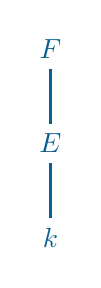
\begin{tikzpicture}
    \draw[thick, figBlue] (0, 0.25) -- (0, 0.95);
    \draw[thick, figBlue] (0, 1.45) -- (0, 2.15);
    \node[inner sep=0.15cm, figBlue] at (0, 2.4) {$F$};
    \node[inner sep=0.15cm, figBlue] at (0, 1.2) {$E$};
    \node[inner sep=0.15cm, figBlue] at (0, 0.0) {$k$};
\end{tikzpicture}
\end{center}
\end{content}

\begin{insight}[Varying Both Vector Spaces and Scalar Fields]
In introductory linear algebra, the ground field of scalars usually acts as a fixed \qt{spectator} throughout an entire course. When working with towers of field extensions $k \subset E \subset F$, both the space of vectors and the field of scalars vary dynamically --- the same field $E$ serves simultaneously as the vector space over $k$ and as the scalar field for $F$.
\end{insight}

\subsection{The Tower Law (Multiplicativity of Degree)}

\begin{speech}[00:21:52 - 00:23:42]
Okay, so, the most basic result in this context is the following proposition \inlinemetanote{writes: Prop:}. Suppose $F$ is finite-dimensional as an $E$-vector space, and $E$ is finite-dimensional as a $k$-vector space --- so, I suppose this --- then (this is the conclusion) you can imagine what I'm going to write: $F$ is finite-dimensional as a $k$-vector space \inlinemetanote{writes \qt{Suppose $F$ is finite dim as $E$-vector space}, \qt{and $E$ is finite dim as $k$-vector space}, \qt{$\Downarrow$ Then}, and \qt{$F$ is finite dim as $k$-vector space}}.

Okay? So, is this logic clear? We're saying if this one \inlinemetanote{points at the $F$--$E$ segment} is finite-dimensional and that's finite-dimensional \inlinemetanote{points at the $E$--$k$ segment}, then the full one \inlinemetanote{points from $k$ to $F$} is finite-dimensional. And this is only part of it, the first one, and the second is that the dimension of $F$ as an $E$-vector space times the dimension of $E$ as a $k$-vector space equals the dimension of $F$ as a $k$-vector space \inlinemetanote{writes: $\dim_E F \cdot \dim_k E = \dim_k F$}.

Okay, so, we're going to prove this, but are there any questions about this statement? It says that if this is finite-dimensional \inlinemetanote{points at $F$--$E$} and that's finite-dimensional \inlinemetanote{points at $E$--$k$}, then this one's finite-dimensional \inlinemetanote{points from $k$ to $F$}, and moreover the dimension here is just the product of the dimensions, that's all. It's a simple result. Yeah?
\end{speech}

\begin{content}
\begin{proposition}[Multiplicativity of Dimension in a Tower]\label[proposition]{prop:tower-law}
Let $k \subset E \subset F$ be a tower of fields. Suppose that:
\begin{enumerate}[label=\textbf{(\arabic*)}]
    \item $F$ is finite-dimensional as an $E$-vector space, and
    \item $E$ is finite-dimensional as a $k$-vector space.
\end{enumerate}
Then $F$ is finite-dimensional as a $k$-vector space, and
\begin{equation}\label{eq:tower-law}
\dim_E F \cdot \dim_k E = \dim_k F.
\end{equation}
\end{proposition}
The dimension $\dim_k E$ is also called the \newterm{degree} of the field extension $k \subset E$; the lecture later speaks of the \qt{degree of the extension} in exactly this sense, and the Tower Law says that degrees multiply in a tower.
\end{content}

\begin{student}[Student Question]
Does this have anything to do with the construction we did before, or is it just...
\end{student}

\begin{speech}[00:23:48 - 00:25:00]
Oh yeah, it's going to come. No, this has nothing... I mean, this is just arbitrary. But we're going to relate it later to the construction we did before. It's a reasonable question. There's no $K$ here, no big $K$ here, but it's going to come later.

All right, so, we try to prove this \inlinemetanote{pushes the lower board up and pulls down the upper boards to erase}. The big $K$ will come later, but I need this result to talk about what's going to happen. And in any case, this result is really kind of like the first result in these towers of vector spaces. And the proof, of course, is simple.

Let us try to prove it. But there's a reasonable question: in these letters there's no big $K$ in this at all \inlinemetanote{erases the boards from the earlier uniqueness discussion}. And no polynomial either.
\end{speech}

\begin{proofWrapper}[Proof of \cref{prop:tower-law}]

\begin{speech}[00:25:01 - 00:26:18]
Okay, so, typically if you want to prove things are finite-dimensional and calculate the dimension, a very straightforward way is to look at bases.

So, the assumptions are that since $F$ over $E$ \inlinemetanote{draws the vertical segment $F$ over $E$} is finite-dimensional, this means we can find a basis \inlinemetanote{writes \qt{finite dim} and \qt{$\Longrightarrow$}}. And since the basis elements are elements of $F$, I write them as $f_1$ to $f_A$, where $A$ is the dimension of $F$ over $E$ \inlinemetanote{writes \qt{$f_1, \dots, f_A \in F$} and \qt{$A = \dim_E F$}}. So, these are all elements of $F$ and these are the basis \inlinemetanote{draws a brace under $f_1, \dots, f_A$ and writes: basis of $F$ as an $E$-vector space}.

So, you're happy with this notation? If it's finite-dimensional, it has some dimension; I call this dimension big $A$, and I find a basis. It's a basis of $F$ as an $E$-vector space. Okay?

All I have done is taken the assumption that this extension's finite-dimensional and used that to pick a basis. Who knows what the basis is, but I can pick it.
\end{speech}

\begin{content}[Choosing a Basis of \texorpdfstring{$F$}{F} over \texorpdfstring{$E$}{E}]
Since $F$ is finite-dimensional as an $E$-vector space, it has some finite dimension $A := \dim_E F$ and admits an $E$-basis
\[
\underbrace{f_1, \dots, f_A}_{\text{basis of } F \text{ as an } E\text{-vector space}} \in F.
\]
\end{content}

\begin{speech}[00:26:18 - 00:27:20]
Similarly, $E$ over $k$ \inlinemetanote{draws the vertical segment $E$ over $k$} is finite-dimensional \inlinemetanote{writes: finite dim $\Longrightarrow$}. So, I can pick --- and now I name the basis elements of this with $e$'s, because they live here --- some $e_1$ to $e_B$ in $E$, where $B$ is equal to the dimension of $E$ over $k$ \inlinemetanote{writes \qt{$e_1, \dots, e_B \in E$} and \qt{$B = \dim_k E$}}. And this is a basis of $E$ as a $k$-vector space \inlinemetanote{draws a brace under $e_1, \dots, e_B$ and writes: basis of $E$ as a $k$-vector space}.

All right, so, all I've done is unpacked; I haven't done anything, I just picked the bases. Now, to be a basis has two properties, of course. There's two properties here: generation and independence \inlinemetanote{draws a fork from the first line labeled \qt{gen} and \qt{indep}}. And there's two properties here: generation and independence \inlinemetanote{draws a fork from the second line labeled \qt{gen} and \qt{indep}}. So, this is what we have: as the assumptions, we have these two bases, and we have the basis properties.
\end{speech}

\begin{content}[Choosing a Basis of \texorpdfstring{$E$}{E} over \texorpdfstring{$k$}{k}]
Similarly, since $E$ is finite-dimensional as a $k$-vector space, it has finite dimension $B := \dim_k E$ and admits a $k$-basis
\[
\underbrace{e_1, \dots, e_B}_{\text{basis of } E \text{ as a } k\text{-vector space}} \in E.
\]
By definition of a basis, each of these two bases satisfies two properties:
\begin{enumerate}[label=\textbf{(\arabic*)}]
    \item \textbf{Over $E$:} $\{f_1, \dots, f_A\}$ generates $F$ over $E$ and is $E$-linearly independent.
    \item \textbf{Over $k$:} $\{e_1, \dots, e_B\}$ generates $E$ over $k$ and is $k$-linearly independent.
\end{enumerate}
\end{content}

\begin{hidden}
% timestamp: 00:27:20
% topic: Proof of the Tower Law (setup of bases for F/E and E/k)
% board_state: prop:tower-law, eq:tower-law
% next_goal: Propose the candidate k-basis {f_i e_j} of F and prove generation and linear independence.
% open_loops: Proof of prop:tower-law in progress.
\end{hidden}

\begin{speech}[00:27:21 - 00:27:57]
Okay, so, we have to now write a basis of $F$ over $k$ \inlinemetanote{writes: Write a basis of $F/k$}.

And you might think the first time: well, maybe we take some of these vectors and maybe put them together, but if we did that we'd get $A + B$, and that's kind of bad because I need to get $AB$ for the answer. So, if I've already told you the answer, then you should probably guess what the answer is here. Can you guess what the basis is going to be? Yeah?
\end{speech}

\begin{student}[Student Answer]
Just all the possible products.
\end{student}

\begin{speech}[00:28:01 - 00:29:43]
Yeah, I mean, the natural way, if you have a set of elements of $A$ and a set of elements of $B$, the natural way to get a set of elements of $AB$ is to take pairs of them, which in this case you can do the product.

So, the proposal here for the basis is this: $f_i e_j$, where $i$ goes from $1$ to $A$ and $j$ goes from $1$ to $B$ \inlinemetanote{writes \qt{Proposal:} and \qt{$\{f_i e_j\} \subset F$ with $1 \le i \le A$ and $1 \le j \le B$}}. Okay?

So, first of all you have to accept that this is a set of vectors in $F$, and the reason it's a set of vectors is $F$ is a field. Here we're thinking about $F$ as a vector space, but $F$ is also a field, so I can take an element of $E$ and multiply it with an element of $F$; it's a legal move, because it's a field. So, this is a construction of some elements here.

And then we have to show that this set here generates $F$ over $k$ and is linearly independent over $k$ \inlinemetanote{writes \qt{We have to show}, \qt{$\{f_i e_j\} \longrightarrow$}, \qt{gen $F/k$}, and \qt{indep/$k$}}. So, we have to show two things for this set, right? That's all we have to do for a basis.

And we have four hypotheses, so we're going to have to use them all. We're going to use these four hypotheses two at a time to get these two.
\end{speech}

\begin{content}[Proposed \texorpdfstring{$k$}{k}-Basis of \texorpdfstring{$F$}{F}]
We propose the following subset of $F$ consisting of $A \cdot B$ pairwise products:
\[
\mathcal{B} := \{ f_i e_j \mid 1 \le i \le A,\; 1 \le j \le B \} \subset F.
\]
(Note that every product $f_i e_j$ lies in $F$ because $E \subset F$ and $F$ is closed under field multiplication.)

To prove that $\mathcal{B}$ is a basis of $F$ as a $k$-vector space, we must verify two claims:
\begin{enumerate}[label=\textbf{(\arabic*)}]
    \item $\mathcal{B}$ generates $F$ over $k$,
    \item $\mathcal{B}$ is linearly independent over $k$.
\end{enumerate}
\end{content}

\begin{speech}[00:29:44 - 00:30:46]
And this proof is really a simple proof. There's no interesting logic or complicated logic. If you say, is there an idea in this proof? The only small idea was that you take the basis here and the basis there and you multiply them together; that's the only idea. Like if you didn't know the answer, then maybe you'd have to think about having the idea, but that's the only idea in the proof. The rest proves itself, but we can do it \inlinemetanote{pushes the current board up and erases the lower board}.
\end{speech}

\subsubsection{Generation over \texorpdfstring{$k$}{k}}

\begin{speech}[00:30:47 - 00:32:08]
So, let's try to prove that it generates \inlinemetanote{writes: gen/$k$}.

This starts with an arbitrary element. So, we start with an element $x$, a totally arbitrary element of $F$ \inlinemetanote{writes: $x \in F$}. All right? And we need to express it in terms of little-$k$-linear multiples of this \inlinemetanote{points at $\{f_i e_j\}$}. So, what are we going to do? How are we going to start?

We have to express $x$ as something, and the only thing we know where we have an $x$ to start with is that we can express $x$ in terms of the $E$-basis, right? It's the only thing we know, right? So, we know we can write $x$ as equal to $f_1$ times some $c_1$ plus $f_2$ times $c_2$ plus $f_A$ times $c_A$, where these $c_i$'s are in $E$ \inlinemetanote{writes \qt{$\longrightarrow x = f_1 c_1 + f_2 c_2 + \dots + f_A c_A$} and \qt{$c_i \in E$}}, right?

Because these $f$'s were the basis, and I can take the linear... Usually we write on the other side, but it doesn't matter; I picked on this side. Okay? Is that okay? Yeah? So, now what do we do? Yeah?
\end{speech}

\begin{student}[Student Answer]
Express the $c$'s in terms of the $e$-basis.
\end{student}

\begin{speech}[00:32:10 - 00:33:54]
Yeah, just express every $c$. Actually, there's really nothing to it. Now you have to take $c_1$, and we use the second... This has used the first generation. Now we use the second generation: $c_1$ is in $E$, so I can express $c_1$ as equal to $e_1$ times... I have to pick another coefficient, okay, $\hat{c}_1$, plus $e_2$ times $\hat{c}_2$ all the way to $e_B$ times $\hat{c}_B$ \inlinemetanote{writes \qt{$c_1 \in E$} and \qt{$c_1 = e_1 \hat{c}_1 + e_2 \hat{c}_2 + \dots + e_B \hat{c}_B$}}. All right?

So, that's the equation for $c_1$. This is an element of $E$, and the hatted coefficients are all elements of $k$ \inlinemetanote{writes: $\hat{c}_i \in k$}. Okay?

And then we just feed this equation in here \inlinemetanote{points at $f_1 c_1$}, and we get $f_1$ times $e_1$, $f_1$ times $e_2$, with coefficients that are in little $k$. All right? And then we do it for all of them, and then we'll just show at the end, if you do that for every one of these, you will have exactly expressed $x$ as a $k$-linear combination of the proposed basis. Okay?

So, this proves generation, and the full generation statement uses the two generation statements above \inlinemetanote{writes \qt{This gen.} with an arrow pointing at the equations, and \qt{Uses 2 gen stat.\ above}}. All right?
\end{speech}

\begin{content}[Proof of Generation over \texorpdfstring{$k$}{k}]
Let $x \in F$ be an arbitrary element.

\textbf{Step 1 (Expand $x$ in the $E$-basis of $F$):} Since $\{f_1, \dots, f_A\}$ generates $F$ as an $E$-vector space, there exist coefficients $c_1, c_2, \dots, c_A \in E$ such that
\[
x = f_1 c_1 + f_2 c_2 + \dots + f_A c_A = \sum_{i=1}^A f_i c_i.
\]

\textbf{Step 2 (Expand each $c_i$ in the $k$-basis of $E$):} Since each $c_i \in E$ and $\{e_1, \dots, e_B\}$ generates $E$ as a $k$-vector space, there exist coefficients $\hat{c}_{i1}, \hat{c}_{i2}, \dots, \hat{c}_{iB} \in k$ such that
\[
c_i = e_1 \hat{c}_{i1} + e_2 \hat{c}_{i2} + \dots + e_B \hat{c}_{iB} = \sum_{j=1}^B e_j \hat{c}_{ij} \qquad (i = 1, \dots, A).
\]
(The board does this for $c_1$, writing $c_1 = e_1 \hat{c}_1 + e_2 \hat{c}_2 + \dots + e_B \hat{c}_B$ with $\hat{c}_j$ for $\hat{c}_{1j}$.)

\textbf{Step 3 (Substitute):} Substituting the expansion of each $c_i$ into the expression for $x$ and using distributivity and associativity in the field $F$ yields
\[
x = \sum_{i=1}^A f_i \left( \sum_{j=1}^B e_j \hat{c}_{ij} \right) = \sum_{i=1}^A \sum_{j=1}^B (f_i e_j) \hat{c}_{ij}.
\]
Since all $\hat{c}_{ij} \in k$, we have expressed $x$ as a $k$-linear combination of $\{f_i e_j\}$. This uses both generation hypotheses and proves that $\{f_i e_j\}$ generates $F$ over $k$.
\end{content}

\subsubsection{Linear Independence over \texorpdfstring{$k$}{k}}

\begin{speech}[00:33:55 - 00:36:15]
So, then we need to prove linear independence \inlinemetanote{writes: lin indep}, and okay. Linear independence is a little bit of a pain because you have to write all these equations out; I never like this part. So, linear independence --- it's better to just think about it than write.

Linear independence: we need to prove this. So, what does linear independence mean? It means you have to consider an arbitrary little-$k$-linear combination of these people, right? What's an arbitrary combination?

It's $f_1 e_1$ --- that's our basis element --- now times some coefficient, and I'll use the hat since I used it there: $f_1 e_1 \hat{c}_{11}$, and then $f_1 e_2$ times $\hat{c}_{12}$, and then $f_2 e_1$ times $\hat{c}_{21}$ \inlinemetanote{writes \qt{$f_1 e_1 \hat{c}_{11}$}, \qt{$+ f_1 e_2 \hat{c}_{12} + \dots$}, and \qt{$+ f_2 e_1 \hat{c}_{21} + \dots$}}.

All right, so, look, it can take a long time to write them all, but everything is plus here. I'm writing them in a matrix --- you could write them in a line, but I'm writing in a matrix for a reason --- so this is the last one, $f_1$ and then $e_B \hat{c}_{1B}$, and then I plus on this side, then we get plus $f_2 e_B \hat{c}_{2B}$ \inlinemetanote{writes \qt{$+ f_1 e_B \hat{c}_{1B}$} and \qt{$+ f_2 e_B \hat{c}_{2B}$}}. Okay, so on, and the last one here has $f_A e_1$ and so on \inlinemetanote{writes: $+ f_A e_1 \dots + f_A e_B \hat{c}_{AB}$}. So, you get a matrix, and this is zero \inlinemetanote{writes: $= 0$}. And all the $\hat{c}_{ij}$'s are in little $k$ \inlinemetanote{writes: $\hat{c}_{ij} \in k$}.

All right, so, that's what you start with for linear independence: you write down an arbitrary linear combination, and to show it's linearly independent, you have to show all these hats are zero --- that's what we have to show, right? So, how are you going to do this?

I wrote it for a reason, right, in this way. \inlinemetanote{waits silently for student responses}

Yeah?
\end{speech}

\begin{content}[Linear Relation in Matrix Layout]
To prove $k$-linear independence of $\{f_i e_j\}$, consider an arbitrary $k$-linear combination set equal to $0$, arranged by rows according to $f_1, \dots, f_A$:
\begin{align*}
  &\phantom{+} f_1 e_1 \hat{c}_{11} + f_1 e_2 \hat{c}_{12} + \dots + f_1 e_B \hat{c}_{1B} \\
  &+ f_2 e_1 \hat{c}_{21} + \dots + f_2 e_B \hat{c}_{2B} \\
  &\phantom{+} \vdots \\
  &+ f_A e_1 \hat{c}_{A1} + \dots + f_A e_B \hat{c}_{AB} = 0,
\end{align*}
where all $\hat{c}_{ij} \in k$. We must show that $\hat{c}_{ij} = 0$ for all $1 \le i \le A$ and $1 \le j \le B$.
\end{content}

\begin{hidden}
% timestamp: 00:36:15
% topic: Proof of the Tower Law (linear independence of {f_i e_j})
% board_state: prop:tower-law, eq:tower-law
% next_goal: Factor out f_i from each row and apply linear independence over E and then over k.
% open_loops: Proof of prop:tower-law nearly complete.
\end{hidden}

\begin{student}[Student Answer]
Factor out $f_1$.
\end{student}

\begin{speech}[00:36:18 - 00:36:44]
Yeah, yeah, this is the reason I wrote it. It took a lot of concentration. There \inlinemetanote{factors out $f_1, f_2, \dots, f_A$ in front of parentheses around each row of the sum}. We factor it out. We've done nothing so far, but we factor it out for every one of these.

Okay, so, all I've done is taken what I wrote and factored out the $f_1$. And that's a thing you can do because it's multiplication. Yeah?
\end{speech}

\begin{student}[Student Question]
Wait, is the last bracket placed correctly?
\end{student}

\begin{speech}[00:36:46 - 00:37:58]
No, it's not, thank you \inlinemetanote{erases the misplaced closing parenthesis and places it to the left of $= 0$}.

So, I factored out, which is a thing you can do because we're talking about fields --- there's all this extra thing of multiplication. Now you look at this, and you interpret it rather as a linear equation in $F$ over $E$ \inlinemetanote{writes $F/E$ to the left of the factored system}, because these are the ones in $F$ and these coefficients are now all in the field $E$.

Then we use the independence --- one of the independences --- the top independence says that these things are linearly independent over $E$. That shows every single coefficient here is zero \inlinemetanote{points at the parenthesized coefficients $e_1 \hat{c}_{i1} + \dots + e_B \hat{c}_{iB}$}. Every single one.

And then for these coefficients themselves, we use the second linear independence: to show that every one of these is zero, we use the second independence, the one of $E$ over $F$ (i.e., $E$ over $k$).

So, that's it. Actually, there's nothing here. It's just, you know, you just have to stay not confused for a few minutes, that's the only thing.
\end{speech}

\begin{content}[Proof of Linear Independence and Conclusion]
Factoring $f_i$ out of the $i$-th row gives
\begin{align*}
  &\phantom{+} f_1 \bigl( e_1 \hat{c}_{11} + e_2 \hat{c}_{12} + \dots + e_B \hat{c}_{1B} \bigr) \\
  &+ f_2 \bigl( e_1 \hat{c}_{21} + \dots + e_B \hat{c}_{2B} \bigr) \\
  &\phantom{+} \vdots \\
  &+ f_A \bigl( e_1 \hat{c}_{A1} + \dots + e_B \hat{c}_{AB} \bigr) = 0.
\end{align*}

\textbf{Step 1 (Apply $E$-linear independence of $\{f_1, \dots, f_A\}$):} Because each $\hat{c}_{ij} \in k \subset E$ and each $e_j \in E$, every parenthesized expression $\sum_{j=1}^B e_j \hat{c}_{ij}$ lies in $E$. Viewing the equation above as an $E$-linear combination of $f_1, \dots, f_A$ in $F$, the $E$-linear independence of $\{f_1, \dots, f_A\}$ implies that every coefficient vanishes:
\[
e_1 \hat{c}_{i1} + e_2 \hat{c}_{i2} + \dots + e_B \hat{c}_{iB} = 0 \qquad \text{for every } i \in \{1, \dots, A\}.
\]

\textbf{Step 2 (Apply $k$-linear independence of $\{e_1, \dots, e_B\}$):} For each fixed $i$, this is a $k$-linear combination of $e_1, \dots, e_B$ in $E$ equal to $0$. Since $\{e_1, \dots, e_B\}$ is linearly independent over $k$, it follows that
\[
\hat{c}_{ij} = 0 \qquad \text{for all } 1 \le i \le A,\; 1 \le j \le B.
\]

\textbf{Conclusion:} Thus, $\{f_i e_j \mid 1 \le i \le A,\; 1 \le j \le B\}$ both generates $F$ over $k$ and is linearly independent over $k$, so it is a $k$-basis of $F$. Moreover, all $A \cdot B$ elements $f_i e_j$ are distinct (if $f_i e_j = f_{i'} e_{j'}$ with $(i, j) \neq (i', j')$, then $f_i e_j - f_{i'} e_{j'} = 0$ would be a $k$-linear relation with coefficients $\hat{c}_{ij} = 1$ and $\hat{c}_{i'j'} = -1$, contradicting $\hat{c}_{ij} = 0$ from Step 2). Therefore, $F$ is finite-dimensional over $k$ and
\[
\dim_k F = A \cdot B = \dim_E F \cdot \dim_k E.
\]
\end{content}

\end{proofWrapper}

\begin{aiNote}[Spoken Slip: \qt{$E$ over $F$}]
% [PERSISTENT]
At 00:37:46, the lecturer says \qt{the one of $E$ over $F$}; he means the linear independence of $e_1, \dots, e_B$ over $k$, that is, $E$ over $k$.
\end{aiNote}

\begin{speech}[00:37:58 - 00:38:08]
So, that's the proof.
\end{speech}

\section{Application: Straightedge and Compass Constructions}

\subsection{Constructible Numbers and Quadratic Towers}

\begin{speech}[00:38:09 - 00:39:59]
All right, so, maybe I give one small example. Probably there's enough time to do it. Let's try to do it quickly \inlinemetanote{pushes the proof board up and erases the lower board}.

So, it has to do with this topic which, you know, used to be popular --- certainly when I was a child it was popular --- which is this kind of straightedge and compass constructions. I don't know whether you know what that is. It was also popular with the ancient Greeks, but that was slightly before my childhood, that.

And the idea with the straightedge and compass is that you have a straightedge and a compass, and the question is what can you construct? And there's a lot of classical impossibility results; the simplest one we can already prove.

So, the straightedge and compass: you have a compass like this \inlinemetanote{draws a V-shaped compass on the far left} and you have a straightedge \inlinemetanote{draws a horizontal line segment below it}, and you're given... that's the plane \inlinemetanote{draws coordinate axes}, and you're given the unit, meaning a unit length \inlinemetanote{marks unit ticks along the axes and draws a square in the first quadrant}. That's the beginning of the story. You have this machine, this compass --- you know what a compass is, right? Do you or not?

And the straightedge, and you start with this unit length, and then you can just do whatever you want with the straightedge and compass. So, you can certainly construct --- I mean, there's a lot of tricks here that you learn somehow --- the easiest thing is you can just fill out the integer points \inlinemetanote{marks equally spaced ticks along the horizontal axis}, and then you can do more things and more...

But the important thing to understand here is that what you're doing when you're doing that is constructing numbers. You can say, like, what points can you construct on the real axis? You're constructing numbers. So, the first numbers you're given are $\mathbb{Z}$, because that's the unit length, and it turns out you can add and subtract, divide numbers, you can construct $\mathbb{Q}$ \inlinemetanote{writes: $\mathbb{Z} \subset \mathbb{Q}$}...
\end{speech}

\begin{content}[Geometric Setup and Constructible Rational Numbers]
In classical straightedge and compass constructions, one begins with a straightedge (unmarked ruler), a compass, and a plane equipped with a given unit length ($1$). Using the compass to step off the unit length along the real axis constructs all integers $\mathbb{Z}$; using straightedge-and-compass constructions for addition, subtraction, multiplication, and division constructs all rational numbers $\mathbb{Q}$:
\[
\mathbb{Z} \subset \mathbb{Q}.
\]

\definecolor{figBlue}{HTML}{07608F} % RGB (7, 96, 143): petrol blue (MidnightBlue)
\definecolor{figGray}{HTML}{666665} % RGB (102, 102, 101): dark gray (gray!80!black)
\definecolor{figOrange}{HTML}{CC7E2A} % RGB (204, 126, 42): ochre orange (BurntOrange!80!black)
\begin{hidden}
- Board (frame 00:44:58): the straightedge is a horizontal line below the compass, so the figure draws it horizontally too.
- Canvas: no scale, cm; left side shows schematic compass (x in [0.0, 1.4]) and straightedge (horizontal, x in [2.0, 3.8] at y = 0.8, label spans ~1.8..4.0 below it), right side shows the coordinate plane with unit length and integer ticks (x in [4.3, 10.7]); y in [-1.5, 2.4]
- Order: (1) compass V-shape and straightedge segment; (2) coordinate axes; (3) unit square and integer ticks; (4) all text last
- Coordinates:
  Compass: apex (0.7, 2.0), legs to (0.1, 0.2) and (1.3, 0.2), hinge circle radius 0.08 at (0.7, 2.0)
  Straightedge: horizontal segment (2.0, 0.8) -- (3.8, 0.8)
  Plane: origin at (6.7, 0), x-axis from (4.3, 0) to (10.5, 0), y-axis from (6.7, -1.2) to (6.7, 2.2)
  Unit step = 1.0 cm: ticks at x = 4.7, 5.7, 7.7, 8.7, 9.7; y = 1.0; unit square (6.7, 0) rectangle (7.7, 1.0)
- Labels (§ Attaching Labels), each with inner sep=0.15cm:
  "compass" anchor north at (0.7, 0.0); "straightedge" anchor north at (2.9, 0.6), 0.2 cm under its bar (closer, the bar read like an overline)
  "0" anchor north east at (6.7, 0.0); "1" anchor north at (7.7, -0.08); "2" anchor north at (8.7, -0.08); "-1" anchor north at (5.7, -0.08)
  "\mathbb{R}" anchor west at (10.5, 0)
- Collisions: "compass" centred at x=0.7 (~0.0..1.4) and "straightedge" centred at x=2.9 (~1.8..4.0) have ~0.4 cm horizontal separation and stop 0.3 cm left of the x-axis at 4.3; tick labels sit below the x-axis; "0" sits in the south-west quadrant clear of both axes.
\end{hidden}
\begin{center}
\begin{tikzpicture}[>=Stealth]
    % (1) Compass and straightedge
    \draw[thick, figGray] (0.1, 0.2) -- (0.7, 2.0) -- (1.3, 0.2);
    \filldraw[fill=white, draw=figGray, thick] (0.7, 2.0) circle (0.08);
    \draw[very thick, figGray] (2.0, 0.8) -- (3.8, 0.8);

    % (2) Coordinate axes
    \draw[->, thick] (4.3, 0) -- (10.5, 0);
    \draw[->, thick] (6.7, -1.2) -- (6.7, 2.2);

    % (3) Unit square and integer ticks
    \draw[thick, figBlue, fill=figBlue!10] (6.7, 0) rectangle (7.7, 1.0);
    \foreach \x in {4.7, 5.7, 7.7, 8.7, 9.7} {
        \draw[thick] (\x, 0.08) -- (\x, -0.08);
    }
    \draw[thick] (6.62, 1.0) -- (6.78, 1.0);

    % (4) Text last
    \node[anchor=north, inner sep=0.15cm, figGray] at (0.7, 0.0) {compass};
    \node[anchor=north, inner sep=0.15cm, figGray] at (2.9, 0.6) {straightedge};
    \node[anchor=north east, inner sep=0.15cm] at (6.7, 0.0) {$0$};
    \node[anchor=north, inner sep=0.15cm] at (5.7, -0.08) {$-1$};
    \node[anchor=north, inner sep=0.15cm, figBlue] at (7.7, -0.08) {$1$};
    \node[anchor=north, inner sep=0.15cm] at (8.7, -0.08) {$2$};
    \node[anchor=west, inner sep=0.15cm] at (10.5, 0) {$\mathbb{R}$};
\end{tikzpicture}
\end{center}
\end{content}

\begin{hidden}
% timestamp: 00:39:59
% topic: Straightedge and compass constructions (setup and constructible numbers)
% board_state: prop:tower-law, eq:tower-law
% next_goal: State the characterization of constructible numbers via towers of degree-2 extensions.
% open_loops: none
\end{hidden}

\begin{speech}[00:39:59 - 00:42:25]
And then, the interesting thing is this compass, because that's the circle \inlinemetanote{draws a circle below the compass}, and a circle satisfies a quadratic equation. So, the answer to what you can construct is: you can construct any number in $\mathbb{R}$ such that --- if I take this number, let's say the number $\alpha$ --- such that $\alpha$ lies in an extension... \inlinemetanote{writes \qt{You can construct}, \qt{any number $\alpha$ in $\mathbb{R}$}, and \qt{such that}, and inserts $\alpha$ after \qt{number}} So, here's $\mathbb{R}$, that's a big thing, and here's $\mathbb{Q}$ \inlinemetanote{draws vertical tower $\mathbb{R}$ over $\mathbb{Q}$}. If I construct it, $\alpha$ lies in some field $E$ \inlinemetanote{adds $E$ on the tower and writes $\alpha \in E$ to its left}.

So, you can construct any $\alpha$ in $E$ such that the dimension of $E$ over $\mathbb{Q}$... Well, let's try to say it correctly: such that $E$ lives in some tower of extensions $F_1$, $F_2$, $F_k$, and then $\mathbb{Q}$, such that every degree of the extension is $2$ \inlinemetanote{writes \qt{Such that} and \qt{$E \subset$}, draws the tower $F_1, F_2, \dots, F_k, \mathbb{Q}$ from the top down, and writes \qt{$2$} beside the steps}.

Did you learn this stuff in high school or not? I don't know. Like I said, it was a kind of a popular topic once. But if you learned it, then this is the conclusion: what can you compute using this? You can compute any number that sits inside an iteration of quadratic extensions.

And the reason is easy, because every time you do this, you're either solving a linear equation --- in which case you don't get out of the field --- or you're solving a quadratic equation, and you can't do anything else. You get the quadratic equation because a circle satisfies a quadratic equation, and a linear equation does nothing. So, there's a little bit to prove, but that's the outcome of just understanding what straightedge and compass construction is: you can compute numbers that come in these quadratic extensions; you can't do anything else. Are you happy with this?
\end{speech}

\begin{content}[Characterization of Constructible Numbers]
A real number $\alpha \in \mathbb{R}$ can be constructed by straightedge and compass if and only if $\alpha$ lies in some subfield $E \subset \mathbb{R}$ such that $E$ is contained in a finite tower of quadratic field extensions starting from $\mathbb{Q}$:
\[
\mathbb{Q} \subset F_1 \subset F_2 \subset \dots \subset F_k, \qquad \text{with } \dim_{\mathbb{Q}} F_1 = \dim_{F_1} F_2 = \dots = \dim_{F_{k-1}} F_k = 2,
\]
and $\alpha \in E \subset F_k$. (The lecture names the fields from the top down, $E \subset F_1$ with $F_k$ just above $\mathbb{Q}$; here they are numbered upwards from $\mathbb{Q}$.)

\definecolor{figBlue}{HTML}{07608F} % RGB (7, 96, 143): petrol blue (MidnightBlue)
\definecolor{figGreen}{HTML}{3D8252} % RGB (61, 130, 82): dark green (ForestGreen!70!black)
\begin{hidden}
- Canvas: no scale, cm; left tower R--E--Q at x = 1.6, right tower F_k--...--F_2--F_1--Q at x = 6.2; x in [0.0, 7.6], y in [-0.4, 4.4]
- Order: (1) tower segments on left and right; (2) all text last
- Coordinates:
  Left tower: Q = (1.6, 0), E = (1.6, 2.0), R = (1.6, 4.0); segments (1.6, 0.25)--(1.6, 1.75) and (1.6, 2.25)--(1.6, 3.75)
  Right tower: Q = (6.2, 0), F_1 = (6.2, 1.0), F_2 = (6.2, 2.0), dots at (6.2, 2.85), F_k = (6.2, 3.8)
  Segments: (6.2, 0.25)--(6.2, 0.75), (6.2, 1.25)--(6.2, 1.75), (6.2, 2.25)--(6.2, 2.55), (6.2, 3.15)--(6.2, 3.55)
- Labels (§ Attaching Labels), each with inner sep=0.15cm:
  "\alpha \in" anchor east at (1.25, 2.0); "E", "\mathbb{R}", "\mathbb{Q}" at left tower centres
  "E \subset" anchor east at (5.8, 3.8) (next to F_k)
  "2" anchor west at (6.3, 0.5), (6.3, 1.5), (6.3, 3.35)
- Collisions: left and right towers are 4.6 cm apart; degree labels "2" sit right of the right tower segments; "\alpha \in" at x=1.25 clears E at x=1.6.
\end{hidden}
\begin{center}
\begin{tikzpicture}[>=Stealth]
    % (1) Left tower: Q subset E subset R
    \draw[thick, figBlue] (1.6, 0.25) -- (1.6, 1.75);
    \draw[thick, figBlue] (1.6, 2.25) -- (1.6, 3.75);

    % (2) Right tower: Q subset F_1 subset F_2 subset ... subset F_k
    \draw[thick, figBlue] (6.2, 0.25) -- (6.2, 0.75);
    \draw[thick, figBlue] (6.2, 1.25) -- (6.2, 1.75);
    \draw[thick, figBlue] (6.2, 2.25) -- (6.2, 2.55);
    \draw[thick, figBlue] (6.2, 3.15) -- (6.2, 3.55);

    % (3) Text last
    \node[inner sep=0.15cm] at (1.6, 4.0) {$\mathbb{R}$};
    \node[inner sep=0.15cm, figBlue] at (1.6, 2.0) {$E$};
    \node[inner sep=0.15cm] at (1.6, 0.0) {$\mathbb{Q}$};
    \node[anchor=east, inner sep=0.15cm, figGreen] at (1.25, 2.0) {$\alpha \in$};

    \node[inner sep=0.15cm, figBlue] at (6.2, 3.8) {$F_k$};
    \node[inner sep=0.15cm, figBlue] at (6.2, 2.85) {$\vdots$};
    \node[inner sep=0.15cm, figBlue] at (6.2, 2.0) {$F_2$};
    \node[inner sep=0.15cm, figBlue] at (6.2, 1.0) {$F_1$};
    \node[inner sep=0.15cm] at (6.2, 0.0) {$\mathbb{Q}$};
    \node[anchor=east, inner sep=0.15cm] at (5.8, 3.8) {$E \subset$};

    \node[anchor=west, inner sep=0.15cm, figGreen] at (6.3, 0.5) {$2$};
    \node[anchor=west, inner sep=0.15cm, figGreen] at (6.3, 1.5) {$2$};
    \node[anchor=west, inner sep=0.15cm, figGreen] at (6.3, 3.35) {$2$};
\end{tikzpicture}
\end{center}

\begin{steps}[Why Only Quadratic Extensions Arise]
Going beyond the lecture: Each new constructible point is obtained by intersecting two lines, a line and a circle, or two circles defined using previously constructed coordinates in a field $F_m$:
\begin{itemize}
    \item \textbf{Line $\cap$ Line:} Solving two linear equations over $F_m$ yields coordinates already in $F_m$ (degree $1$).
    \item \textbf{Line $\cap$ Circle:} Substituting a linear equation into a quadratic circle equation $(x - a)^2 + (y - b)^2 = r^2$ (with $a, b, r^2 \in F_m$) yields a quadratic equation over $F_m$. By the quadratic formula, its solutions lie in $F_m$ if its discriminant $d \in F_m$ has a square root in $F_m$, and otherwise in the degree-$2$ extension $F_{m+1} = F_m(\sqrt{d})$.
    \item \textbf{Circle $\cap$ Circle:} Subtracting the two circle equations cancels the $x^2$ and $y^2$ terms, reducing the system to a line $\cap$ circle intersection.
\end{itemize}
By the Tower Law (\cref{prop:tower-law}), iterating $k$ such steps yields a field $F_k$ of dimension $\dim_{\mathbb{Q}} F_k = 2^k$ over $\mathbb{Q}$.
\end{steps}
\end{content}

\begin{aiNote}[Beyond the Lecture: The Field \texorpdfstring{$E$}{E} and Degrees That Are Powers of \texorpdfstring{$2$}{2}]
% [PERSISTENT, ADDITION]
For $E$ one may always take $\mathbb{Q}(\alpha)$, the smallest subfield of $\mathbb{R}$ containing $\alpha$ (\cref{def:subfield-generated-by-beta}), since it lies in every subfield of $\mathbb{R}$ that contains $\alpha$. By the Tower Law for $\mathbb{Q} \subset \mathbb{Q}(\alpha) \subset F_k$, $\dim_{\mathbb{Q}} \mathbb{Q}(\alpha)$ then divides $2^k$, so it is a power of $2$. This condition is necessary but not sufficient: there are real numbers $\alpha$ with $\dim_{\mathbb{Q}} \mathbb{Q}(\alpha) = 4$ that cannot be constructed (Galois theory shows this). This is why the characterization asks for a tower of quadratic steps, and not only for a dimension.
\end{aiNote}

\subsection{Impossibility of Trisecting an Angle}

\begin{speech}[00:42:25 - 00:43:24]
So, then the traditional first application of this is that it's impossible to trisect angles \inlinemetanote{writes: Imposs.\ to trisect angles} --- meaning you cannot trisect any angle. And the standard angle that's used for this is that you take the angle $60^\circ$ \inlinemetanote{writes: $60^\circ$}. That's the angle for the equilateral triangle \inlinemetanote{draws an equilateral triangle below $60^\circ$}, and you can ask: could I construct the trisector of that?

The trisector of $60^\circ$ would be a $20^\circ$ angle \inlinemetanote{writes: $\longrightarrow 20^\circ$}. And if you study what you can do here, if you could trisect this angle, that means you could construct this $20^\circ$. That means you could construct this number: cosine of $20^\circ$ \inlinemetanote{writes: $\cos(20) = \alpha$}. That would mean cosine of $20^\circ$ is this $\alpha$ \inlinemetanote{points back to $\alpha$}. You would have to be able to construct this cosine of $20^\circ$...
\end{speech}

\begin{content}[Reduction of Angle Trisection to \texorpdfstring{$\cos(20^\circ)$}{cos(20 degrees)}]
A classical impossibility result is that one cannot trisect an arbitrary angle with straightedge and compass. As a concrete counterexample, consider an angle of $60^\circ$ (which is constructible, as it is the interior angle of an equilateral triangle: the circles of radius $1$ around the two ends of the unit segment meet in its third vertex):
\[
60^\circ \longrightarrow 20^\circ.
\]
If $60^\circ$ could be trisected, one could construct a $20^\circ$ angle at the end $0$ of the unit segment, and by dropping a perpendicular from the point at distance $1$ on its ray onto the horizontal unit segment, one could construct the length $\alpha = \cos(20^\circ) \in \mathbb{R}$.

\definecolor{figBlue}{HTML}{07608F} % RGB (7, 96, 143): petrol blue (MidnightBlue)
\begin{hidden}
- Canvas: no scale, cm; equilateral triangle of side 2.0 on [0, 2.0] x [0, 1.732]; x in [-0.4, 2.4], y in [-0.4, 2.1]
- Order: (1) equilateral triangle (0,0)--(2,0)--(1,1.732)--cycle; (2) 60 deg angle arc at (0,0) of radius 0.45; (3) label last
- Coordinates: top vertex (1, 1.732); arc from 0 to 60 deg at radius 0.45; label 60^\circ at (30:0.85) = (0.736, 0.425) inside the triangle
- Collisions: label at (0.736, 0.425) sits 0.425 cm from both adjacent sides, 0.40 cm outside the arc at r=0.45, and 0.88 cm from the opposite side.
\end{hidden}
\begin{center}
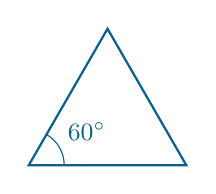
\begin{tikzpicture}
    \draw[thick, figBlue] (0, 0) -- (2, 0) -- (1, 1.732) -- cycle;
    \draw[figBlue] (0.45, 0) arc (0:60:0.45);
    \node[inner sep=0.15cm, figBlue, font=\small] at (30:0.85) {$60^\circ$};
\end{tikzpicture}
\end{center}
\end{content}

\begin{speech}[00:43:24 - 00:45:01]
Now I just have to write down one more equation. So, what is this cosine of $20^\circ$? Well, there's this triple-angle formula, if you remember from high school --- actually, do I remember it? --- so, $3\theta$ (i.e., $\cos(3\theta)$) is equal to $4 \cos(\theta)^3 - 3 \cos(\theta)$ \inlinemetanote{writes: $\cos(3\theta) = 4 \cos^3(\theta) - 3 \cos(\theta)$}. That's the triple-angle formula, which you should remember from high school.

And if you put it here \inlinemetanote{points at $\cos(3\theta)$}, if you put $\theta = 20^\circ$, cosine of $3\theta$ is cosine of $60^\circ$, that's a half --- you should remember that also. And so, it says that a half is $4$ times the cosine of $20^\circ$ (cubed) minus $3$ times the cosine of $20^\circ$ \inlinemetanote{writes: $\frac{1}{2} = 4 \cos^3(20) - 3 \cos(20)$}.

So, this gives an equation for the cosine of $20^\circ$, and it's a cubic equation. And you can then actually check it's irreducible --- I don't do that now, it's elementary to check that this cubic equation over the rationals is irreducible. So, the cosine of $20^\circ$ satisfies an irreducible cubic equation.

So, wherever it sits, we can find our $K$ --- it's finally come back to the $K$! Since it's a solution of this, we can find the $K$ in here \inlinemetanote{draws a diagonal link from $\mathbb{Q}$ to $K$ inside the $\mathbb{Q} \subset E \subset \mathbb{R}$ tower, labeled $3$}, and this $K$ has degree $3$ --- the one that's the minimal $\alpha$ (i.e., the minimal field containing $\alpha$). And a $3$ can never be a divisor of a power of $2$; that's the proof, actually! Yeah, that's the proof. Okay, good, that's it.

I did finish, barely.
\end{speech}

\begin{content}[Cubic Equation and Contradiction via the Tower Law]
Recall the triple-angle trigonometric identity:
\[
\cos(3\theta) = 4 \cos(\theta)^3 - 3 \cos(\theta).
\]

\begin{steps}[Deriving the Triple-Angle Formula]
Going beyond the lecture: under multiplication of complex numbers the angles add (\cref{fact:pre-complex}), so $\cos(3\theta) + i \sin(3\theta) = (\cos(\theta) + i \sin(\theta))^3$. Comparing real parts gives $\cos(3\theta) = \cos(\theta)^3 - 3 \cos(\theta) \sin(\theta)^2 = 4 \cos(\theta)^3 - 3 \cos(\theta)$, using $\sin(\theta)^2 = 1 - \cos(\theta)^2$.
\end{steps}

Setting $\theta = 20^\circ$ and using $\cos(3 \cdot 20^\circ) = \cos(60^\circ) = \frac{1}{2}$ gives
\[
\frac{1}{2} = 4 \cos(20^\circ)^3 - 3 \cos(20^\circ).
\]
Thus, $\alpha = \cos(20^\circ)$ is a root of the cubic polynomial $f(x) = 8x^3 - 6x - 1 \in \mathbb{Q}[x]$ (equivalently $x^3 - \frac{3}{4}x - \frac{1}{8}$), which is irreducible over $\mathbb{Q}$.

Suppose toward a contradiction that $\alpha = \cos(20^\circ)$ were constructible, so $\alpha \in E \subset F_k$ for some tower of quadratic extensions $\mathbb{Q} \subset F_1 \subset \dots \subset F_k$. By the uniqueness of the construction (\cref{thm:uniqueness-root-extension}), the smallest subfield $K \subset E$ containing $\alpha$ is isomorphic to $\faktor{\mathbb{Q}[x]}{(f)}$ by an isomorphism that is the identity on $\mathbb{Q}$, hence $\mathbb{Q}$-linear, so by \cref{prop:dim-quotient-field} its dimension over $\mathbb{Q}$ is
\[
\dim_{\mathbb{Q}} K = \operatorname{degree}(f) = 3.
\]
Now consider the tower $\mathbb{Q} \subset K \subset F_k$. The field $F_k$ is finite-dimensional over $K$, since a $\mathbb{Q}$-basis of $F_k$ spans $F_k$ over $K$ as well. By the Tower Law (\cref{prop:tower-law}):
\[
\dim_{\mathbb{Q}} F_k = \dim_K F_k \cdot \dim_{\mathbb{Q}} K = \dim_K F_k \cdot 3,
\]
so $3 \mid \dim_{\mathbb{Q}} F_k$. On the other hand, applying the Tower Law iteratively along $\mathbb{Q} \subset F_1 \subset \dots \subset F_k$ gives $\dim_{\mathbb{Q}} F_k = 2^k$. Since $3$ can never divide a power of $2$, this is a contradiction. Therefore, $\cos(20^\circ)$ is not constructible, and an angle of $60^\circ$ cannot be trisected with straightedge and compass.

\definecolor{figBlue}{HTML}{07608F} % RGB (7, 96, 143): petrol blue (MidnightBlue)
\definecolor{figRed}{HTML}{B5241C} % RGB (181, 36, 28): brick red (BrickRed)
\definecolor{figGreen}{HTML}{3D8252} % RGB (61, 130, 82): dark green (ForestGreen!70!black)
\begin{hidden}
- Canvas: no scale, cm; left side shows the subfield K inside E over Q inside F_k/R; right side shows the quadratic tower; x in [-0.4, 7.6], y in [-0.4, 4.4]
- Order: (1) main tower Q--E--R and right tower Q--F_1--F_2--...--F_k; (2) branch Q--K--E in figRed; (3) text last
- Coordinates:
  Left: Q = (1.8, 0), E = (1.8, 2.2), R = (1.8, 4.0); K = (0.4, 1.1)
  Segments: (1.8, 0.25)--(1.8, 1.95), (1.8, 2.45)--(1.8, 3.75)
  Branch Q->K: vector (-1.4, 1.1), unit (-0.786, 0.618); segment (1.58, 0.17)--(0.63, 0.91)
  Branch K->E: vector (1.4, 1.1), unit (0.786, 0.618); segment (0.64, 1.29)--(1.57, 2.01)
  Right: Q = (6.2, 0), F_1 = (6.2, 1.0), F_2 = (6.2, 2.0), dots (6.2, 2.85), F_k = (6.2, 3.8)
- Labels (§ Attaching Labels), each with inner sep=0.15cm:
  "3" by auto on (1.58, 0.17)--(0.63, 0.91) (since the path goes up-and-left, auto places "3" below-left, outside the Q--K--E triangle)
  "K" at (0.4, 1.1) in figRed
  "E \subset" anchor east at (5.8, 3.8)
  "2" anchor west at (6.3, 0.5), (6.3, 1.5), (6.3, 3.35)
- Collisions: K sits at x = 0.4, 1.4 cm left of the Q--E axis; "3" sits outside the Q--K--E triangle.
\end{hidden}
\begin{center}
\begin{tikzpicture}[>=Stealth]
    % (1) Left tower R -- E -- Q and Right tower F_k -- ... -- Q
    \draw[thick, figBlue] (1.8, 0.25) -- (1.8, 1.95);
    \draw[thick, figBlue] (1.8, 2.45) -- (1.8, 3.75);
    \draw[thick, figBlue] (6.2, 0.25) -- (6.2, 0.75);
    \draw[thick, figBlue] (6.2, 1.25) -- (6.2, 1.75);
    \draw[thick, figBlue] (6.2, 2.25) -- (6.2, 2.55);
    \draw[thick, figBlue] (6.2, 3.15) -- (6.2, 3.55);

    % (2) Subfield K of degree 3
    \draw[thick, figRed] (1.58, 0.17) -- (0.63, 0.91);
    \draw[thick, figRed] (0.64, 1.29) -- (1.57, 2.01);

    % (3) Text last
    \node[inner sep=0.15cm] at (1.8, 4.0) {$\mathbb{R}$};
    \node[inner sep=0.15cm, figBlue] at (1.8, 2.2) {$E$};
    \node[inner sep=0.15cm] at (1.8, 0.0) {$\mathbb{Q}$};
    \node[inner sep=0.15cm, figRed] at (0.4, 1.1) {$K$};
    \path (1.58, 0.17) -- (0.63, 0.91) node[midway, auto, inner sep=0.15cm, figRed] {$3$};

    \node[inner sep=0.15cm, figBlue] at (6.2, 3.8) {$F_k$};
    \node[inner sep=0.15cm, figBlue] at (6.2, 2.85) {$\vdots$};
    \node[inner sep=0.15cm, figBlue] at (6.2, 2.0) {$F_2$};
    \node[inner sep=0.15cm, figBlue] at (6.2, 1.0) {$F_1$};
    \node[inner sep=0.15cm] at (6.2, 0.0) {$\mathbb{Q}$};
    \node[anchor=east, inner sep=0.15cm] at (5.8, 3.8) {$E \subset$};
    \node[anchor=west, inner sep=0.15cm, figGreen] at (6.3, 0.5) {$2$};
    \node[anchor=west, inner sep=0.15cm, figGreen] at (6.3, 1.5) {$2$};
    \node[anchor=west, inner sep=0.15cm, figGreen] at (6.3, 3.35) {$2$};
\end{tikzpicture}
\end{center}

\begin{steps}[Verifying Irreducibility of \texorpdfstring{$8x^3 - 6x - 1$}{8x\textasciicircum 3 - 6x - 1} over \texorpdfstring{$\mathbb{Q}$}{Q}]
Going beyond the lecture: A cubic polynomial over $\mathbb{Q}$ is reducible if and only if it has a linear factor, i.e., a rational root. Suppose $f(\frac{p}{q}) = 0$ with $p, q \in \mathbb{Z}$, $q > 0$ and $(p, q) = 1$; here $p \neq 0$, since $f(0) = -1$. Multiplying by $q^3$ gives $8p^3 - 6pq^2 - q^3 = 0$, so $p$ divides $q^3 = 8p^3 - 6pq^2$. A prime factor of $p$ would then divide $q$ (Euclid's lemma, \cref{fact:pre-euclid}), which is impossible since $(p, q) = 1$; so $p = \pm 1$. Then $q$ divides $8p^3 = \pm 8$, so $q \in \{1, 2, 4, 8\}$. This leaves only the candidates $\pm 1, \pm \frac{1}{2}, \pm \frac{1}{4}, \pm \frac{1}{8}$. Evaluating directly:
\begin{align*}
f(\pm 1) &= \pm 8 \mp 6 - 1 \in \{1, -3\}, & f\!\left(\pm \frac{1}{2}\right) &= \pm 1 \mp 3 - 1 \in \{-3, 1\}, \\
f\!\left(\pm \frac{1}{4}\right) &= \pm \frac{1}{8} \mp \frac{3}{2} - 1 \in \left\{-\frac{19}{8}, \frac{3}{8}\right\}, & f\!\left(\pm \frac{1}{8}\right) &= \pm \frac{1}{64} \mp \frac{3}{4} - 1 \in \left\{-\frac{111}{64}, -\frac{17}{64}\right\}.
\end{align*}
None of these vanishes, so $8x^3 - 6x - 1$ has no rational root and is therefore irreducible over $\mathbb{Q}$.
\end{steps}
\end{content}

\begin{overview}[Summary of Key Concepts]
\begin{itemize}
    \item \textbf{Dimension of a Simple Quotient Extension:} For a field $k$ and an irreducible polynomial $f \in k[x]$ of degree $d$, the field $K = \faktor{k[x]}{(f)}$ is a finite-dimensional $k$-vector space with basis $\{\bar{1}, \bar{x}, \dots, \bar{x}^{d-1}\}$ and $\dim_k K = \operatorname{degree}(f)$.
    \item \textbf{Uniqueness up to Isomorphism:} For any field extension $F$ of $k$ containing a root $\beta$ of $f$, the universal property of $k[x]$ gives a unique evaluation homomorphism $\phi \colon k[x] \to F$ with $\phi|_k = \operatorname{Id}_k$ and $\phi(x) = \beta$. Its kernel is $(f)$, inducing an isomorphism $\bar{\phi} \colon K \xrightarrow{\sim} \operatorname{Im}(\phi) \subset F$ onto the smallest subfield of $F$ containing $k$ and $\beta$.
    \item \textbf{The Tower Law:} For a tower of fields $k \subset E \subset F$ where $F$ is finite-dimensional over $E$ (with basis $\{f_1, \dots, f_A\}$) and $E$ is finite-dimensional over $k$ (with basis $\{e_1, \dots, e_B\}$), the products $\{f_i e_j\}$ form a $k$-basis of $F$, giving $\dim_E F \cdot \dim_k E = \dim_k F$.
    \item \textbf{Impossibility of Angle Trisection:} A real number $\alpha$ is constructible by straightedge and compass if and only if it lies in a subfield $E \subset F_k$ of a finite tower $\mathbb{Q} \subset F_1 \subset \dots \subset F_k$ of degree-$2$ extensions (since lines give degree-$1$ equations and circles give quadratic equations). Since $\cos(20^\circ)$ satisfies an irreducible cubic equation over $\mathbb{Q}$ (from $\cos(3\theta) = 4\cos(\theta)^3 - 3\cos(\theta)$), it generates a degree-$3$ subfield $K$, which cannot sit inside a field of degree $2^k$ over $\mathbb{Q}$. Hence, $60^\circ$ cannot be trisected.
\end{itemize}
\end{overview}